\documentclass{report}

%------------------------------------------------------------
% All packages are here defined
%------------------------------------------------------------
%\usepackage{mathtools}
\usepackage[table]{xcolor}
\usepackage[a4paper]{geometry}
\usepackage{vmargin}
\usepackage[english]{babel}
\usepackage[english]{varioref}
\usepackage[utf8]{inputenc}
\usepackage{graphicx}
\usepackage{array}
\usepackage{float}
\usepackage{tabularx}
\usepackage{hhline}
\usepackage{amsmath}
\usepackage{amssymb}
\usepackage{hyperref}
\usepackage{url}
\usepackage{fancyhdr}
\usepackage{setspace}
\usepackage{listings}
\usepackage{color}
\usepackage{abstract}
\usepackage{titlesec}
\usepackage{multirow}
\usepackage{datetime}
\usepackage{varwidth}
%\usepackage{svg}
\usepackage{epsfig}
\usepackage{blindtext}
\usepackage{xcolor}
\usepackage{enumitem}
%----------------------------------------------------
%	MARGINS
%----------------------------------------------------
\setmarginsrb  { 1.5in}  % left margin
                        { 0.6in}  % top margin
                        { 1.0in}  % right margin
                        { 0.8in}  % bottom margin
                        {  20pt}  % head height
                        {0.25in}  % head sep
                        {   9pt}  % foot height
                        { 0.3in}  % foot sep
%----------------------------------------------------------------------------------------

%-------------------------------------------------
% Colors defination
%--------------------------------------------------
\definecolor{dkgreen}{rgb}{0,0.6,0}
\definecolor{gray}{rgb}{0.5,0.5,0.5}
\definecolor{mauve}{rgb}{0.58,0,0.82}
\definecolor{navyblue}{rgb}{0.0, 0.0, 0.5}



%-------------------------------------------------
% JAVA language settings for code insertion
%---------------------------------------------------
\lstset{frame=tb,
  language=Java,
  aboveskip=3mm,
  belowskip=3mm,
  showstringspaces=false,
  columns=flexible,
  basicstyle={\small\ttfamily},
  numbers=none,
  numberstyle=\tiny\color{gray},
  keywordstyle=\color{blue},
  commentstyle=\color{dkgreen},
  stringstyle=\color{mauve},
  breaklines=true,
  breakatwhitespace=true,
  tabsize=3,
  captionpos=b
  %numbers=left,                    % where to put the line-numbers; possible values are (none, left, right)
  %numbersep=10pt
}

%----------------------------------------------------------
% Horizontal line formation
%--------------------------------------------------------
\newcommand{\Hline}{\par
  \begin{center}
   \line(1,0){400}
   \end{center}
}


%------------------------------------------------------
% heading formation for chapters and other headings
%------------------------------------------------------
\titleformat
{\chapter} % command
[display] % shape
{\bfseries\LARGE} % format
{\Huge{Chapter.\ \thechapter}} % label
{0.5ex} % sep
{
\rule{\textwidth}{1pt}%
\vspace{1ex}
\centering
} % before-code
[
\vspace{-0.5ex}%
\rule{\textwidth}{0.3pt}
] % after-code

%-------------------------------------------------------
%heading formation for Acknowledgement
%-------------------------------------------------------


%---------------------------------------------------------
% Others
%----------------------------------------------------------

\newdateformat{mydate}{\monthname[\THEMONTH] \THEYEAR}	
%\geometry{a4paper}
\renewcommand{\abstractnamefont}{\normalfont\LARGE\bfseries}


%------------------------------------------------------
% Beginning main document
%---------------------------------------------------

\begin{document}
\pagenumbering{gobble} 


%----------------------------------------------------------------------------------------
%	Title page
%----------------------------------------------------------------------------------------
\begin{titlepage}
\begin{center}


{\huge \bfseries Graph Theoretical Algorithms For }\\[0.3cm]
{\huge \bfseries Structural Comparison Of Java Source}\\[0.3cm] % Thesis title
{\huge \bfseries  And Byte Code }\\[0.3cm]
\Hline

\begin{center}
\large{Submitted By}\\[0.2cm]
\textbf{\Large{Artem Garishin}}\\[2cm]
\end{center}


\includegraphics[width=0.50\textwidth]{Figures/FH_logo}\\[0.5cm]
\textbf{\large FB2: Faculty of Computer Science and Engineering}\\[1cm]


\large \textit{This thesis presented for the degree of\\ Master of Science} \\
\textit{in the}\\[0.2cm]
\textbf{\textcolor{navyblue}{High Integrity Systems}}\\[2.5cm] % Research group name and department name

\begin{center}


\begin{varwidth}{0.8\textwidth}
\raggedright
\textbf{Research Supervisor}: {Prof. Dr. Sergej Alekseev}\\[0.2cm] % Supervisor name - remove the \href bracket to remove the link  
\textbf{Co-Supervisor}: {Prof. Dr. Matthias Wagner}\\ % Supervisor name - remove the \href bracket to remove the link  
[3cm]
\end{varwidth}\\[3cm]
\end{center}



{\large \mydate\today}\\[1cm] % Date
%\includegraphics{Logo} % University/department logo - uncomment to place it

\vfill

\end{center}

\end{titlepage}


%----------------------------------------------------------
%Declaration
%---------------------------------------------------------
%\doublespacing%
\onehalfspacing
\null\vfil
%\vskip 60\p@
\begin{center}{\huge\bf Legal Declaration\par}\end{center}
%\vskip 60\p@
\null
I declare that this thesis document is completely my own work and all used references have been clearly cited. I have not submitted this assignment in the context of an examination to any other examination board or person.\\[2.5cm]

\begin{flushleft}
Signature:\\
\rule[1em]{25em}{0.5pt} % This prints a line for the signature
 
Location, Date:\\
\rule[1em]{25em}{0.5pt} % This prints a line to write the date
\end{flushleft}


%-----------------------------------------------------------------
% Abstract 
%----------------------------------------------------------
\newpage
\pagestyle{fancy}
\fancyhead{}
\renewcommand{\headrulewidth}{0pt}
\renewcommand{\footrulewidth}{0.4pt}
\pagenumbering{Roman}
%\doublespacing
\begin{abstract}
\large

TODO:
\par 
This should be a 1-page (maximum) summary of your work. What environment for development has been used, experimental results 
An abstract is a summary in your own words of the Thesis It is not evaluative and must not include your personal opinions. The purpose of an abstract is to give a reader sufficient information for him or her to decide whether it would be worthwhile reading the entire article or book. An abstract should aim at giving as much information as possible in as few words as possible. 
\par 
Goal of this work is to search out the most optimal ways to compare different pieces of code. So far there are two techniques for code comparison: a normal text comparison and visual compare. Normal text-compare can be not sufficient to analyse two pieces of code, or to find a similarity between them. For that reason a structural/graph compare opens a doors to discover more possibilities of comparison. 

\end{abstract}

%--------------------------------------------------------
%Acknowledgement
%-------------------------------------------------------
\newpage
%\null\vfil
%\vskip 60\p@
\begin{center}{\huge\bf Acknowledgments\par}\end{center}
%\vskip 60\p@
\null
I would like to take this time to thank Frankfurt University of Applied Sciences for all of the resources which they provided me in order to pursuing my master study in computer science and make this thesis possible.\vspace{5 mm}

\noindent I would like to express my sincere gratitude to Prof. Dr. Sergej Alekseev and Prof. Dr. Matthias Wagner for their patient guidance, encouragement and advice which they provided me throughout this thesis work.

%----------------------------------------------------------------------
% Some configurations
%-------------------------------------------------------

\newpage
\tableofcontents
\listoffigures
\listoftables

%--------------------------------------------------------
%Abbreviations
%-------------------------------------------------------
\newpage
\setstretch{1.5}
%\null\vfil
%\vskip 60\p@
\Hline
\begin{center}{\huge\bf Abbreviations\par}\end{center}
\Hline
%\vskip 60\p@
\vspace{10mm}
\null

\noindent
\textbf{TDMC} \hspace{20 mm} \textbf{T}op \textbf{D}own \textbf{M}ax \textbf{C}ommon \\
\textbf{BUMC} \hspace{20 mm} \textbf{B}ottom \textbf{U}p \textbf{M}ax \textbf{C}ommon \\
\textbf{BCV} \hspace{24 mm}  \textbf{B}yte \textbf{C}ode \textbf{V}isualizer \\
\textbf{SCV} \hspace{25 mm}  \textbf{S}ource \textbf{C}ode \textbf{V}isualizer \\
\textbf{CFGF} \hspace{22 mm} \textbf{C}ontrol \textbf{F}low \textbf{G}raph  \textbf{F}actory \\
\textbf{TC} \hspace{27 mm}   \textbf{T}ext \textbf{C}ompare \\
\textbf{MBM} \hspace{22 mm} \textbf{M}aximum \textbf{B}ipartite \textbf{M}atching \\

%------------------------------------------------------
% Example chapter
%------------------------------------------------------

%\chapter{Example}
%\section{Section}
%This is section heading
%\subsection{Sub Section}
%This is sub section

%------------------------------------------------------
% 1st Chapter Introduction
%------------------------------------------------------

\newpage
\pagenumbering{arabic}
\onehalfspacing
\large

\chapter{Introduction}

Modern methods to compare of programming pieces of code are used to analyze code's changing, to explore development process and so on. Basically in current tools or plug-ins only text compare methods are used, that is not full sufficient to define code compare.
Sometimes another techniques can be very helpful for such purposes. One of them is a structural code compare, based on building a trees, and methods to compare any similar or same structures. 

TODO START:
You can't write a good introduction until you know what the body of the paper says. Consider writing the introductory section(s) after you have completed the rest of the paper, rather than before.
Be sure to include a hook at the beginning of the introduction. This is a statement of something sufficiently interesting to motivate your reader to read the rest of the paper, it is an important/interesting scientific problem that your paper either solves or addresses. You should draw the reader in and make them want to read the rest of the paper. 

REDO:
Code duplication or copying a code fragment and then reuse by pasting with or
without any modifications is a well known code smell in software maintenance. Several
studies show that about 5 to 20 percent of a software systems can contain duplicated code,
which is basically the results of copying existing code fragments and using then by
pasting with or without minor modifications. One of the major shortcomings of such
duplicated fragments is that if a bug is detected in a code fragment, all the other
fragments similar to it should be investigated to check the possible existence of the
same bug in the similar fragments. Refactoring of the duplicated code is another prime
issue in software maintenance although several studies claim that refactoring of certain
clones are not desirable and there is a risk of removing them. However, it is also widely
agreed that clones should at least be detected.

Code duplicates represent a common problem for all the
software systems and especially for the large ones, in the
same time being a sign of bad design [1]. The analysis of
the software systems has proven that a considerable
amount of the source code is duplicated. According to [2],
5-10 pre of the source code consists of duplicated code and
according to [3] this percentage rises to 13-18 pre. The main
reason for which code clones appear is the way the
programmers understand to reuse code. They tend to
directly copy fragments of code that implement something
similar to their needs and by performing small changes
they adapt it to the new context and that piece of code is
reused. Another reason for which programmers duplicate
code is presented in [4]: it is easier and faster to copy a
code fragment (which may be already tested) than writing
the code from scratch. As presented in [5], the occurrence
of software clones has many different causes: reusing
code by copying existing idioms, coding styles,
instantiations of definitional computations, failure to
identify or use abstractions, performance enhancement,
accidents.

REDO


Tips:
A statement of the goal of the paper: why the study was undertaken, or why the paper was written. Do not repeat the abstract. 

TODO: Similarity to FreeBSD, Linux, and NetBSD Systems  + Grafik

%-----------------------------------------------------
% 2nd Chapter: Description of problem
%-----------------------------------------------------
\newpage	
\chapter{Description of problem}
\label{cha:Description}

In this chapter an issue of the master work is being explained. As usual a compare of two code fragments consider comparison of classes, functions or methods. Thereby a compare can be counted as examinations of two pieces of code, in the best case a methods or functions. They can have a similar implementation or alike syntax, however these two pieces of code are different.

There are many purposes to compare a code, to find out a similarity or determine a difference between them. One of the option is to search for plagiarism in case a code can be taken from external source and a variables have been changed. In addition to general search can be improved to look out a similar code in big projects. 
\\
REDO: Duplicated code occurs frequently in real programs,as indicated by the results of several studies
\\
Structural compare stands for comparing two graphs. There are many possibilities how to create a graph from java source. In order to find some structural similarities this two created graphs must be compared. For this purpose there are existing algorithms to figure out graph isomorphism. For example the maximum common sub-tree isomorphism algorithms. The purpose of them to seek out the largest common sub-tree between two trees. These algorithms are used not only to investigate code difference but also they are a fundamental problem with multiplicity of applications in nature sciences and engineering.
But unfortunately it is possible only for trees but not for graphs. If two graphs are being isomorphic compared with each other, then it is an NP - complete problem and takes much times and efforts to be done. 

%TODO: write what is NP-complete, write a problems with time execution
In the complex theory the worst case running time of all known algorithms is of exponential order, and just for certain special types of graphs, polynomial-time algorithms have been devised\cite{graph_isomorphism_is}.Maximum common sub-graph isomorphism is an optimization problem that is known to be NP-hard. The formal description of the problem is as follows:
There are two input graphs, respectively the maximum common sub-graph isomorphism MCSGI($ G_{1}, G_{2}$):

\begin{itemize}
	\item     Input: Two graphs $ G_{1}$ and $G_{2}$.
	\item     Question: What is the largest sub-graph of  $ G_{1}$ isomorphic to a sub-graph of  $ G_{2}$ can be found?
\end{itemize}

The associated decision problem, i.e., given $ G_{1}$, $ G_{2}$ and an integer $k$, deciding whether $ G_{1}$ contains a sub-graph of at least $k$ edges isomorphic to a sub-graph of $ G_{2}$ is NP-complete\cite{graph_isomorphism_is}.This type of graph comparison is very expensive from a computational point of view and thus, and some action must be taken into account to reduce the domain of comparison before performing the actual comparison. Therefore this problem must to be reduced. Luckily, a tree comparison is able to executed in polynomial time and moreover there are some existing algorithms to compare trees.

Thus there are no deterministic algorithms to compare them because of loops in graphs. In this case the input code can be transformed into graph firstly, after the graph creation, it must be converted into tree, using simple techniques removing back edges. The back edges in the input graph are edges, which point from a node to one of its ancestors. Under those circumstances the following techniques are searched and deployed in the paper.
After all a few questions can be asked:
\begin{enumerate}
  \item How to transform code into tree by optimal way?
  \item How to compare these trees to get reasonable results?
  \item How to reference code pieces and nodes, respectively how to put the code difference by the most elegant way?
\end{enumerate}

Regards to the first question, the concept of idea is described in chapter \textbf{Graphs Transformation} \ref{cha:graph-transformation}. The second question comprehends existing algorithm and their combination and improvements in chapter \textbf{Existing algorithms} \ref{cha:algorithms-to-compare}. The very last issue is about how to lead back the result of the code and is stated in chapter.

Possible result of this thesis is development of concept to find out code difference using graph theory, in the best case a tool in Project Dr. Garbage \cite{drgarbage}. Can be implemented that highlights similarity/difference of input code snippet and represented respective graph.

To get started with a small example demonstrating, what kind of result gives text compare (text-to-text compare):

\begin{lstlisting}
		public void method1(){
		if(i > 1) i++;
	}
	
	public void method2(){
		if(i > 1) 
		i++;
	}

\end{lstlisting}
	
In this example, two pieces of code there one enter symbol after line (i > 1). The result therefore the codes look different. Using simple text compare approach, only these gap will be found, however this difference does not play any role regards business-logic. In Abstract Syntax View, these two graphs will be same, and no discrepancy will have been discovered.
\begin{figure}[h]
  \centering
  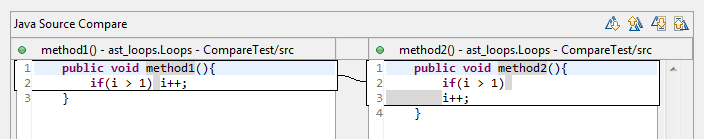
\includegraphics[scale=0.6]{Figures/introduction/intro-code-example}\\[0.1cm]
  \caption[Text to text comparison example]{The simplest example of text-to-text comparison indicating that text compare sometimes is not enough to investigate code difference, however there are no changes regards the application logic}
  \label{fig:intro-code-example}
\end{figure}

	
Since this article includes comparison not only of source code, but also Java byte code, where there is no syntax. Basically to have a look at byte code example, there are no bounds to hold a functions or methods. Based on this, control flow graph can be derived from byte code, that represents a graph, but not a spanning tree. Every node has a reference to byte code address.

%TODO: is any idea how to optimize spanning tree(node has a byte code address, topologically sort)

%TODO: find java bytecode example and his tree

%IDEA: text difference highlight and in parallel nodes in Tree marks and Matching
%(TODO: make some experiments, if it's ok, better, worse or same compare)

%EDIT:
To investigate code comparison, two algorithms of structural compare are required, in fact top-down maximum common sub-tree and bottom-up maximum common sub-tree algorithms. To make a contribution into development of structured code compare, the following tasks should be explored:

\begin{enumerate}
  \item The existing algorithms must be investigated (The text-compare method is not sufficient to find a similarity in code)
  \item The algorithms for the structured compare(Abstract syntax trees, Control flow graphs) must be explored 
  \item New methods and algorithms find a place to tried out. A prototypes of combination text-compare and structure-compare can be implemented.
  \item Experimental results of compare must be derived.
\end{enumerate}
%EDIT

%-----------------------------------------------------
% 3nd Chapter: Graphs comparisons algorithms
%-----------------------------------------------------
\chapter{Tree isomorphism algorithms}
\label{cha:algorithms-to-compare}

This chapter is concerned with the issue of an important generalization of tree isomorphism, mostly known as Maximum Common Sub-tree isomorphism. The goal of these algorithms is finding a largest common sub-tree between two trees. It plays a major role either in scientific fields or in fundamental problems. The trees can be searched for most common sub-tree from top to down, correspondingly form the head of tree till leaves, or from bottom to up, that means the search for largest sub-tree starts from leaves upwards. The algorithms are provided by Gabriel Valiente \cite{valiente}. In his book \emph{Algorithms on Trees and Graphs} he presented detailed information about Top Down Max Common Sub-tree and Bottom Up Max Common Sub-tree isomorphism. The algorithms have been implemented in dr. Garbage tools for plugin eclipse integrated development environment. 

Further research in this area may include not only the implementation of algorithms but also their application field. On this grounds, that the algorithms can be very helpful for tree similarity investigation. The current chapter includes an explanation of how these two algorithms have implemented in the project, about auxiliary algorithms and how they can be helpful for code comparison.

\section{Top-down maximum common sub-tree isomorphism algorithm}
\label{sec:topdown}

There are two types of top-down maximum common sub-tree isomorphism algorithms. One of them finds the largest common ordered sub-tree $T$ between $ T_{1}$ and $ T_{2}$ such can found in both trees, by that when the sequence of edges from parent node does make a sense. On the contrary, the second type is the same top-down algorithm that takes into account the order of edges of parent node, during the algorithm execution. 

A top-down common sub-tree of two unordered trees $ T_{1}$ and $ T_{2 }$ is an unordered tree $T$ such that there are top-down unordered sub-tree isomorphisms of $ T$ into $ T_{1}$ and into $ T_{2}$. A maximal top down common sub-tree of two unordered  trees $ T_{1}$ and $ T_{2}$ is a top-down common sub-tree of $ T_{1}$ and $ T_{2}$ which is not a proper sub-tree of any other top-down common sub-tree of $ T_{1}$ and $ T_{2}$. A top-down of two unordered trees $ T_{1}$ and $ T_{2}$ is a top-down common sub-tree of $ T_{1}$ and $ T_{2}$ with the largest number of nodes \cite{valiente}.

\textbf{Definition 3.1}. \emph{
A \textbf{top-down common sub-tree} of an unordered tree $ T_{1} = ( V_{1}, E_{1})$ to another unordered tree $ T_{2} = ( V_{2}, E_{2})$ is a structure 
$ (X_{1}, X_{2}, M)$, where $ X_{1} = (W_{1}, S_{1})$ is a top down unordered subtree of $ T_{2}$ and $M \subseteq W_{1} \times  W_{2}$ is an ordered tree isomorphism of $ X_{1}$ to $ X_{2}$. A top-down common sub-tree $ (X_{1}, X_{1}, M)$ of $ T_{1}$ to $ T_{2}$ is \textbf{maximal} if there is no top-down common sub-tree of $ (X_{1}', X_{2}', M')$ of $ T_{1}$ to $ T_{2}$ such that $ X_{1}$  is a proper top-down common sub-tree of $ X_{1}'$ and $ X_{2}'$ is a proper top-down sub-tree of $ X_{2}'$, and it is \textbf{maximum} if there is no top-down common sub-tree $ (X_{1}', X_{2}', M')$  of $ T_{1}$ to $ T_{2}$ with the $size[X_{1}] < size[X_{1}']$\cite{valiente}.
}

%PICTURE TDMC
\begin{figure}[hb]
  \centering
  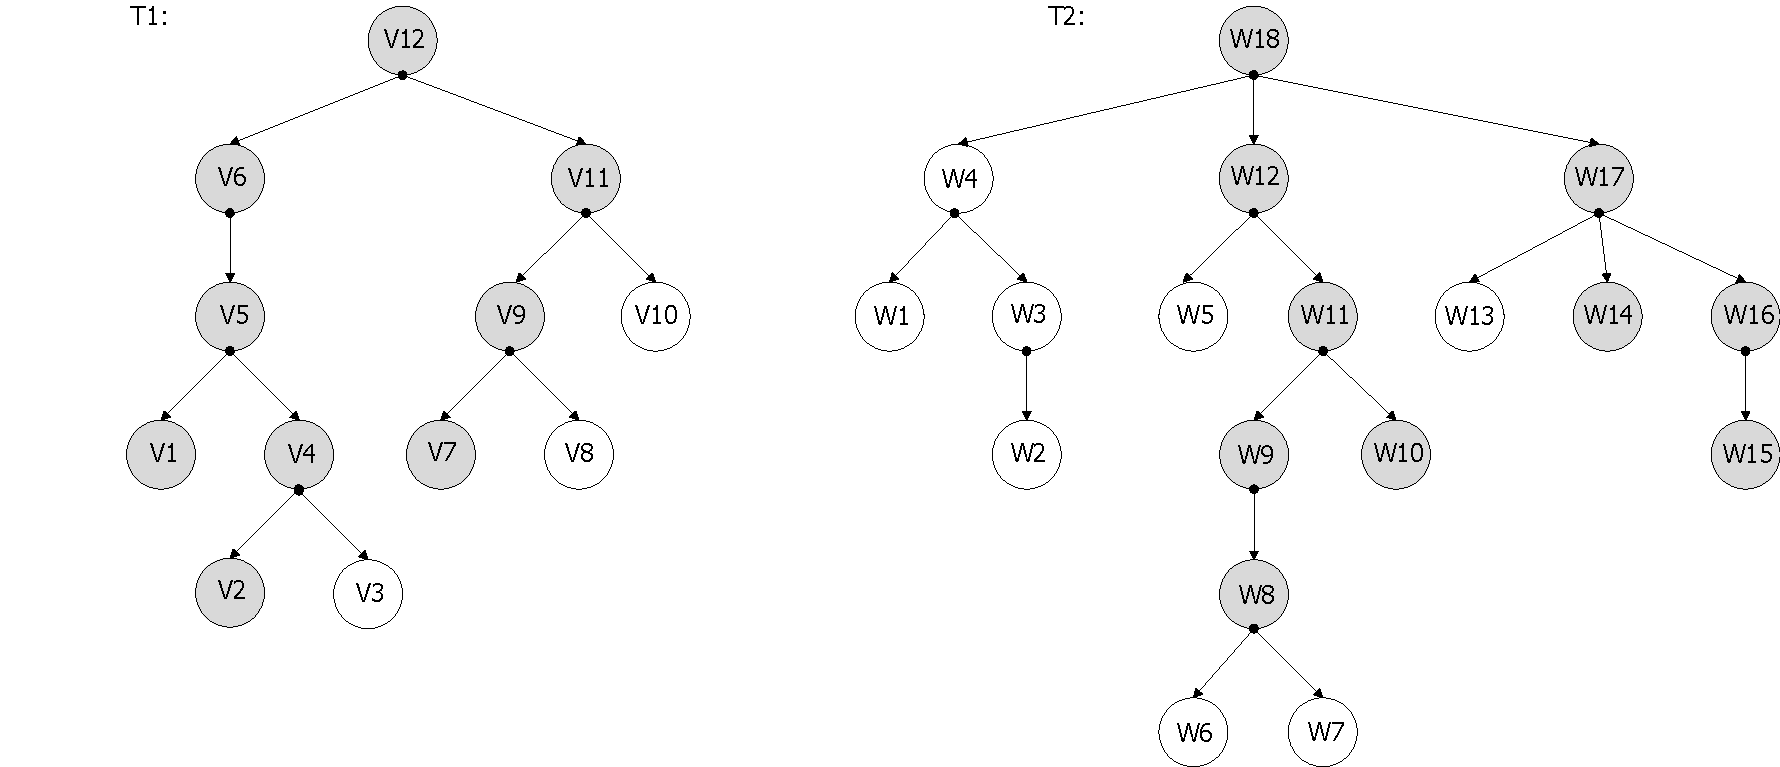
\includegraphics[scale=0.45]{Figures/algorithms/TD/top-down-max-common-example-adjusted.pdf}\\[0.1cm]
  \caption[Top-down maximum common ordered sub-tree of two unordered trees T1 and T2]{Top-down maximum common ordered sub-tree of two unordered trees T1 and T2. Nodes are numbered according to the order in which they are visiting during a post order traversal. The gray highlighted nodes are shaped maximum common sub-tree starting from the root \cite{valiente}.}
  \label{fig:top-down-max-common-example-adjusted}
\end{figure}

The figure \ref{fig:top-down-max-common-example-adjusted} demonstrates a partial injection $M \subseteq W_{1} \times  W_{2}$ among trees $ T_{1} = ( V_{1}, E_{1})$ and  $ T_{2} = ( V_{2}, E_{2})$ where $M  = \{ (v1,w10),  (v2,w8), (v4,w9), $ \\
$(v5,w11),  (v6,w12),  (v7,w15),  (v9,w16), $  $ (v10,w14),  (v11,w17),  (v12,w18)\}$ is unordered top-down maximum common sub-tree isomorphism $ T_{1}$ and $ T_{2 }$ \cite{valiente}.

Important to realize that the injection $M \subseteq W_{1} \times  W_{2}$ can contain different pairs of nodes, as a result there are is only one unique maximum common sub-tree available. Nevertheless the number of pairs of nodes is constant and always maximal.

If nodes $v$ is leaf $ T_{1}$ and $w$ is leaf of $T_{2 }$ accordingly mapped to each other, then the maximum common sub-tree gains size 1. Let suppose that $p$ is number of children of $ T_{1}$ and $q$ is number of children of $ T_{2}$ respectively. Consequently $ v_{1},...,v_{p}$ and $ w_{1},...,w_{q}$ are children of 
 $v$  and $w$\cite{valiente}. Solving the algorithm needs to build a bipartite graph $G=(\{v_{1},...,v_{p}, w_{1},...,w_{q} \}, E)$ on $p+q$ vertices, with edge 
$ v_{i},w_{i} \in E$  if and only if the size of maximum common sub-tree of the sub-tree $ T_{1}$ rooted at node $ v_{i}$ and the sub-tree of $T_{2 }$ rooted at node $ w_{i}$ is non zero\cite{valiente}. 
The bipartite graphs are built recursively the algorithm in one of trees $ T_{1}$ or $ T_{2}$ a leaf reaches. Let the leaf node of $ v_{i}$ of tree $ T_{1}$ is found, then a bipartite graph can be formed with node $ w_{i}$ from $ T_{2}$ at the same hierarchy level. Using the algorithm of \emph{Maximum Bipartite Matching} the corresponding parent nodes $ w_{i+1}$ and $ v_{i+1}$ gains weight one plus \emph{Maximum Bipartite Matching}(in short, MBM)of current bipartite graph.

%PIC 1
\begin{figure}
  \begin{minipage}[h]{0.60\linewidth}
    \centering
    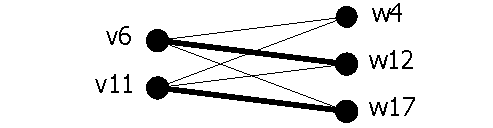
\includegraphics[scale=0.95]{Figures/algorithms/TD/1ex.pdf}\\[0.1cm]
    
  \end{minipage}%
  \begin{minipage}[b]{0.30\linewidth}
    \centering
\begin{tabular}{|c|c|c|c|}
\hline
    & w4 & w12                       & w17                       \\ \hline
v6  & 3  & \cellcolor[gray]{0.9} 5 & 3                         \\ \hline
v11 & 4  & 5                         & \cellcolor[gray]{0.9}4 \\ \hline
\end{tabular}
\end{minipage}
\caption{The solution MBM of bipartite graph brings $5+4=9$ weight from previous solutions}
\label{fig:ex1}
\end{figure}
%PIC 1

%PIC 3
\begin{figure}[h]
  \begin{minipage}[h]{0.60\linewidth}
    \centering
    
\includegraphics[scale=0.95]{Figures/algorithms/TD/3ex.pdf}\\[0.1cm]
  \end{minipage}%
  \begin{minipage}[h]{0.30\linewidth}
    \centering
\begin{tabular}{|c|c|}
\hline
   & w2 \\ \hline
v1 &  \cellcolor[gray]{0.9}1  \\ \hline
v4 & 1  \\ \hline
\end{tabular}
\end{minipage}
\caption{The $v_{1}$ and $v_{4}$ are leaf nodes of the left branch of $ T_{1}$, and leaf node $w_{2}$ of $ T_{2}$. The edge $(v_{1},v_{4})$ is selected with \emph{MBM} algorithm. }
\label{fig:ex3}
\end{figure}
%PIC 3

%PIC 2
\begin{figure}
  \begin{minipage}[h]{0.60\linewidth}
    \centering
    
\includegraphics[scale=0.95]{Figures/algorithms/TD/2ex.pdf}\\[0.1cm]
  \end{minipage}%
  \begin{minipage}[b]{0.30\linewidth}
    \centering
	\caption{}
\begin{tabular}{|c|c|c|}
\hline
   & w1 & w3                        \\ \hline
v5 & 1  & \cellcolor[gray]{0.9} 2 \\ \hline
\end{tabular}
\end{minipage}
\caption{The edge $(v_{5},v_{3})$ gains weight equal to two from previous solution\ref{fig:ex3}, due to the parent node}
\label{fig:ex2}
\end{figure}
%PIC 2

As an example can be taken from figure \ref{fig:ex1}. As said, the nodes are being traversed until leaf node in the trees $ T_{1}$ or $ T_{2}$ is found. Let consider the left branch of $ T_{1}$, namely leaves $v_{1}$ and $v_{4}$ and respectively the left branch of $ T_{2}$, namely leaf $w_{2}$. A created bipartite graph is depicted at figure  \ref{fig:ex3}. The corresponding table shows weights of edges. Since these two are leaves they equal one. With algorithms \emph{MBM} the edge $v_{1}$ and $w_{2}$ is being selected. Once the selection is done, the algorithm take their parent nodes, accordingly $v_{5}$, $w_{3}$ and $v_{3}$. The appropriate bipartite graph is constructed. The edges  $v_{5}$ and $w_{3}$ have weight equal to one initially in table \ref{fig:ex2}, but since from previous solution \ref{fig:ex3}  the node $v_{1}$ has a parent $v_{5}$, the edge $(v_{5},w_{3})$ gets weight equal to two. Likewise the edge  $(v_{6},w_{4})$ in table \ref{fig:ex1} has a value three based on previous result.

By the same way all entries in table \ref{fig:ex1} have been built. Passing through the tree $ T_{1}$ at another left branch until leaves $v_{2}$ and $w_{3}$ the similar bipartite graph can be formed \ref{fig:ex6}. As said before, the current edges get same weight equal to one. The edge $(v_{2},w_{8})$ is selected regards the \emph{MBM} algorithm. Under those circumstances the next bipartite graph can be built \ref{fig:ex5}. Based on previous solution the edge $(v_{4},w_{9})$ obtains weight equal to two.

%PIC 6
\begin{figure}[h]
  \begin{minipage}[h]{0.60\linewidth}
    \centering
    
\includegraphics[scale=0.95]{Figures/algorithms/TD/6ex.pdf}\\[0.1cm]
  \end{minipage}%
  \begin{minipage}[b]{0.30\linewidth}
    \centering
\begin{tabular}{|c|c|}
\hline
   & w8 \\ \hline
v2 & \cellcolor[gray]{0.9} 1  \\ \hline
v3 & 1  \\ \hline
\end{tabular}
\end{minipage}
\caption{Starting from leaves select of both trees select edges with maximum weight. According to the algorithm the connection $(v_{2},w_{8})$ has been selected.}
\label{fig:ex6}
\end{figure}
%PIC 6

%PIC 5
\begin{figure}[h]
  \begin{minipage}[h]{0.60\linewidth}
    \centering
    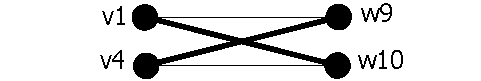
\includegraphics[scale=0.95]{Figures/algorithms/TD/5ex.pdf}\\[0.1cm]
    
  \end{minipage}%
  \begin{minipage}[b]{0.30\linewidth}
    \centering
\begin{tabular}{|c|c|c|}
\hline
   & w9 & w10 \\ \hline
v1 & 1  & \cellcolor[gray]{0.9} 1   \\ \hline
v4 &  \cellcolor[gray]{0.9}2  & 1   \\ \hline
\end{tabular}
\end{minipage}
\caption{Since previous decision was $(v_{2},w_{8})$, and they respectively are parents of $(v_{4},w_{9})$ its weight of edge gains one plus the decision equal to one.}
\label{fig:ex5}
\end{figure}
%PIC 5

%PIC 4
\begin{figure}[h]
  \begin{minipage}[h]{0.60\linewidth}
    \centering
    
\includegraphics[scale=0.95]{Figures/algorithms/TD/4ex.pdf}\\[0.1cm]
    
  \end{minipage}%
  \begin{minipage}[b]{0.30\linewidth}
    \centering
\begin{tabular}{|c|c|c|}
\hline
   & w5 & w11 \\ \hline
v5 & 1  &  \cellcolor[gray]{0.9} 4   \\ \hline
\end{tabular}
\end{minipage}
\caption{The the sum maximum matched edges from \ref{fig:ex5} equal to 3, in the same manner the edge $(v_{5},w_{11})$ gains 3 + 1 = 4 weight}
\label{fig:ex4}
\end{figure}
%PIC 4

Having a look at table in \ref{fig:ex1} in cell $(v_{6},w_{12})$ where the value is 5. This has been formed due to the solution from table \ref{fig:ex4}, because nodes $(v_{6},w_{12})$ are direct parents of $(v_{5},w_{11})$. likewise all other leaves in both trees are investigated and on-fly the tables with weight are filled out. The table in \ref{fig:ex1} is completed by the same way as described above. At the end the maximum bipartite matching algorithm selects the edges $(v_{6},w_{12})$ and $(v_{11},w_{17})$ because they bring the maximum weight of the bipartite graph. In this case two branches in \ref{fig:top-down-max-common-example-adjusted} are picked and the corresponding nodes are grey highlighted forming the maximum common sub-tree from the bottom.
Pseudo code is represented  below:

\begin{lstlisting}
list<node, node> topDownMaxCommonSubtreeIsomorphism(const TREE T1, const TREE T2){
node r1 = root(T1);
node r2 = root(T2);
traverse(node r1, node r2);
M = list<node, node>
reconstruct(r1, M);
}
\end{lstlisting}

This method goes recursively simultaneously through T1 and T2 till leaves of them are founded.
\begin{lstlisting}
void traverse(node v, node w){
int p = v.getNumberOfChildren();
int q = w.getNumberOfChildren();
if(p == 0 or q == 0) return 1;

Array matrix = new Array[p][q];

for(i = 0; i < p; i++){
	for(j = 0; j < q; j++){
		node vChild = v.getChild();	
		node wChild = w.getChild();
		matrix[i][j] = <vChild, wChild, -1>
	}
}

int res = 1;
if(p != 0 and q != 0){
bipartiteGraph bg = createBipartiteGraphFromMatrixEntry(matrix);
if (bg.numberOfEdges == 0) return 0;

list<edge> L = MaxWeightedBipartiteMatching(bg);
forall(e, L){
result += e.getCounter();
}
matching(list<edge> L);
return res;
}
}
\end{lstlisting}
This method reconstructs the top-down max common unordered sub-tree isomorphism mapping.
\begin{lstlisting}
reconstruct(node r1, list<node, node> M){
M[r1] = r2;
list<node> L;
preorder-tree-traversal(L, T1);
forall(node v, L){
	forall(node w, B[v]){
	if(M[T1.parent(v)] == T1.parent(w)){
		M[v] = w;
		break;	
	}
}
}
\end{lstlisting}
%TODO: redo this code
Puts into list B matched edges for further reconstruction
\begin{lstlisting}
matching(list<edge> L){
forall(e, L){
B[r1].insert(r2);
}
}
\end{lstlisting}

\section{Bottom-Up maximum common sub-tree isomorphism algorithm }
\label{sec:bottomup}

There are two types of bottom-up maximum common sub-tree isomorphism algorithms. One of them finds the largest common ordered sub-tree $T$ between $ T_{1}$ and $ T_{2}$ such can found in both trees, by that when the sequence of edges from parent node does make a sense. On the contrary, the second type is the same top-down algorithm that takes into account the order of edges of parent node, during the algorithm execution. 

A bottom-up common sub-tree of two unordered trees $ T_{1}$ and $ T_{2 }$ is an unordered tree $T$ such that there are top-down unordered sub-tree isomorphisms of $ T$ into $ T_{1}$ and into $ T_{2}$. A maximal bottom-up common sub-tree of two unordered  trees $ T_{1}$ and $ T_{2}$ is a bottom-up common sub-tree of $ T_{1}$ and $ T_{2}$ which is not a proper sub-tree of any other bottom-up common sub-tree of $ T_{1}$ and $ T_{2}$. A bottom-up of two unordered trees $ T_{1}$ and $ T_{2}$ is a bottom-up common sub-tree of $ T_{1}$ and $ T_{2}$ with the largest number of nodes \cite{valiente}.

\textbf{Definition 3.1}. \emph{
A \textbf{bottom-up common sub-tree} of an unordered tree $ T_{1} = ( V_{1}, E_{1})$ to another unordered tree $ T_{2} = ( V_{2}, E_{2})$ is a structure 
$ (X_{1}, X_{2}, M)$, where $ X_{1} = (W_{1}, S_{1})$ is a bottom-up unordered subtree of $ T_{2}$ and $M \subseteq W_{1} \times  W_{2}$ is an ordered tree isomorphism of $ X_{1}$ to $ X_{2}$. A bottom-up common sub-tree $ (X_{1}, X_{1}, M)$ of $ T_{1}$ to $ T_{2}$ is \textbf{maximal} if there is no bottom-up common sub-tree of $ (X_{1}', X_{2}', M')$ of $ T_{1}$ to $ T_{2}$ such that $ X_{1}$  is a proper bottom-up common sub-tree of $ X_{1}'$ and $ X_{2}'$ is a proper bottom-up sub-tree of $ X_{2}'$, and it is \textbf{maximum} if there is no bottom-up common sub-tree $ (X_{1}', X_{2}', M')$  of $ T_{1}$ to $ T_{2}$ with the $size[X_{1}] < size[X_{1}']$\cite{valiente}.
}

%PICTURE OF BUMC
\begin{figure}[th]
  \centering
  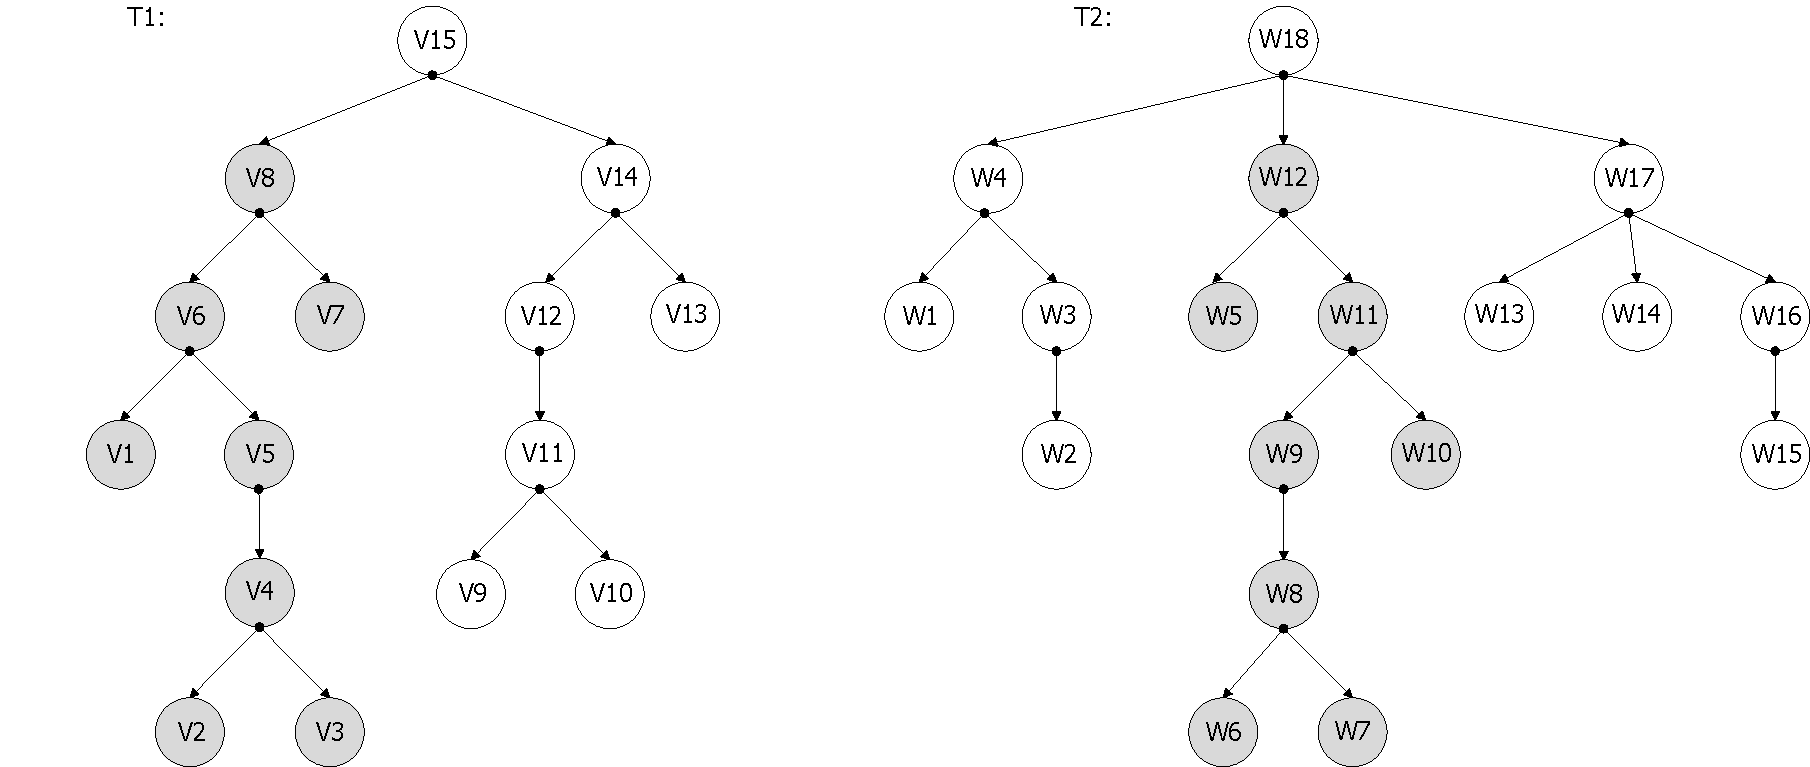
\includegraphics[scale=0.45]{Figures/algorithms/BU/bottom-up-max-common-example.pdf}\\[0.1cm]
  \caption[Bottom Up maximum common ordered sub-tree of two unordered trees T1 and T2]{Bottom Up maximum common ordered sub-tree of two unordered trees T1 and T2. Nodes are numbered according to the order in which they are visiting during a post order traversal. The gray highlighted nodes are shaped maximum common sub-tree starting from the leaves \cite{valiente}.}
  \label{fig:bottom-up-max-common-example}
\end{figure}

The figure \ref{fig:bottom-up-max-common-example} demonstrates a partial injection $M \subseteq W_{1} \times  W_{2}$ among trees $ T_{1} = ( V_{1}, E_{1})$ and  $ T_{2} = ( V_{2}, E_{2})$ where $M  = \{ (v1,w10),  (v2,w6), (v3,w7), $ \\
$(v4,w8),  (v5,w9),  (v6,w11),  (v7,w5), $  $ (v8,w12)\}$ is unordered bottom-up maximum common sub-tree isomorphism $ T_{1}$ and $ T_{2 }$ \cite{valiente}.

The problem of finding a maximum common sub-tree isomorphism between two trees $ T_{1}$ and $ T_{2 }$, where $ T_{1}$ has $n_{1}$ nodes and $ T_{2}$ has $n_{2}$ respectively can be reduced to the problem of partitioning $ V_{1}\bigcup V_{2}$ into equivalent classes of bottom-up sub-tree isomorphism. Two nodes are equivalent if and only if the bottom-up unordered sub-tree rooted at them are isomorphic.

The algorithm start with a partition a tree into bottom-up equivalence classes.
Let the number of known equivalence classes be initially equal to 1, corresponding to the equivalence class of all leaves in the trees. For all nodes v of $ T_{1}$ and $ T_{2 }$ in post-order, set the equivalence class of $V$ to 1 if node $v$ is a leaf. Otherwise, look up in the dictionary the ordered list of equivalent classes to which the children of node $v$ belong. If the ordered list (key) is found in the dictionary then set the equivalence class off node $v$ to the value (element) found. Otherwise, increment by one the number of known equivalence classes, insert the ordered list together with the number of known equivalence classes in the dictionary, and set the equivalence class of node $v$ to the number of known equivalence classes.

\begin{figure}[th]
  \centering
  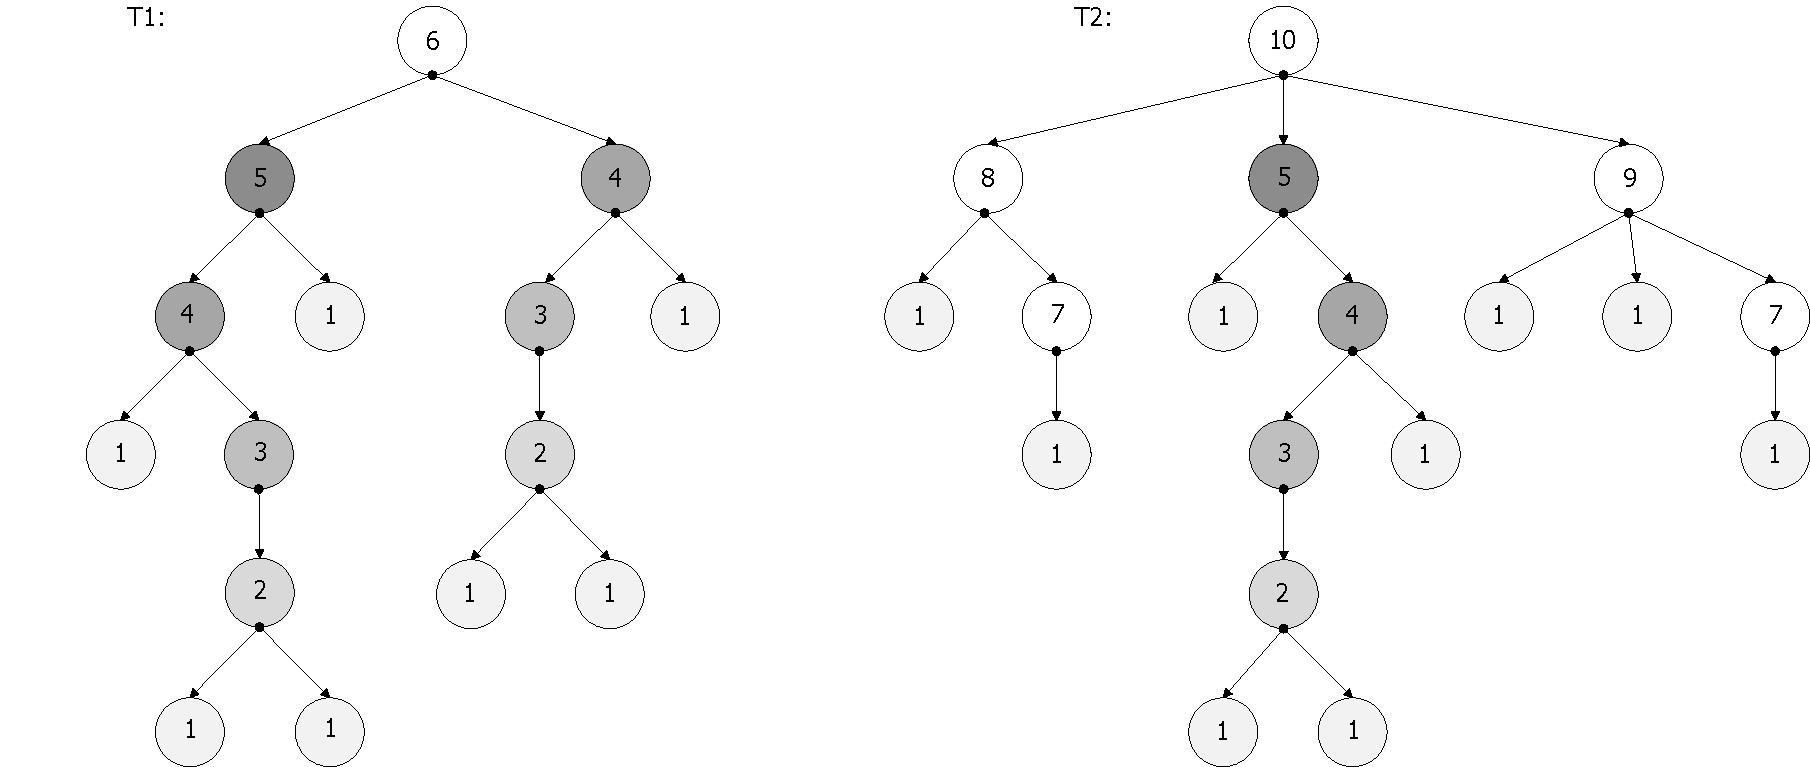
\includegraphics[scale=0.45]{Figures/algorithms/BU/bottom-up-max-common-example-equivalence.pdf}\\[0.1cm]
  \caption[Bottom Up maximum common equivalence classes for figure.] { Bottom Up maximum common equivalence classes reflected to the figure \ref{fig:bottom-up-max-common-example}. The node are numbered according to the equivalence class to which they belong and the equivalence classes are shown highlighted in the different shades of gray\cite{valiente}.}
  \label{fig:bottom-up-max-common-example-equivalence}
\end{figure}

%-----------------------------------------------------
% 4th Chapter: Code compare experiments
%-----------------------------------------------------

\chapter{Code compare experiments}
\label{cha:experimental}
\section{Introduction to experiments}

For better understanding of possible "code compare" concept, possible ideas of implementation and following development an amount of experiments are required.
In order to build a proper tool or at least a concept, in Eclipse plugins at Dr. Garbage Community\textregistered \enspace some hand experiments in code should be fulfilled.

All these test cases are performed in Eclipse IDE \cite{eclipse_site} and divided into blocks. These steps can be approached by following:

\begin{enumerate}
  \item Research on Java source code using existing methods to compare:
  	\begin{enumerate}
   	 	\item Normal text compare
   		 \item Spanning trees transformed from control flow graphs
	 \end{enumerate}	
	 
  \item Research on Java source code using existing methods to compare:
  \begin{enumerate}
    \item Normal text compare 
    \item Abstract syntax trees
  \end{enumerate}
  
  \item Research on Java byte code using existing methods to compare:
  \begin{enumerate}
    \item Normal text compare 
    \item Control flow graphs
  \end{enumerate}
\end{enumerate}

All test set are investigated under Java methods and functions. Playing around with the patterns of code changing variables, names, sequences of commands, adding loops or conditions and apply the simple "text to text" compare. This comparison is already implemented in Eclipse IDE \cite{eclipse_site}, so-called command "compare with each other by member". This type of comparison provides a pop-up window, where two pieces of code are compared, line by line.


In parallel a control flow graphs or source graphs from the functions are being created and compared using implemented algorithms Top-Down and Bottom-Up(following called: TD\& BU). The further task is to figure out the difference/similarity from graphical visual comparison. Consequently these both results must be matched and recorded for succeeding research.

The derived results from can be as follows: 
\begin{enumerate}
  \item Text compare and TD \& BU have same difference
  \item Text compare and TD \& BU give similar difference
  \item Text compare and TD \& BU five full difference
\end{enumerate}

Hence, as it was declared in section description of problem, based on these results can be decided what kind of tool in Dr. Garbage Eclipse plug-ins can be built.In case similar or full difference results, a combination of both methods can be used for optimal comparison. 

Small example can be demonstrated: there are two functions that look very similar but nevertheless they have different number of string and different functionality. The abstract results can be following:
\begin{enumerate}
	\item Text compare shows that strings 1 and 5 are different
	\item Graph compare shows that string 7 is different 
\end{enumerate}

Conclusion: a combination of two methods can explicit that strings 1,5 and 7 are distinguished and much more distinction has been found. Thus it provides an optimal way of investigation.


% JAVA SOURCE CODE EXPERIMENTS

\section{Experiments on Java source code Flowcharts}

A flowchart is a type of diagram that represents an algorithm, workflow or process, showing the steps as boxes of various kinds, and their order by connecting them with arrows. This diagrammatic representation illustrates a solution model to a given problem. Flowcharts are used in analyzing, designing, documenting or managing a process or program in various fields\cite{wiki_flowchart}.

Dr. Garbage tools\cite{drgarbage} provides a solution how to represent sequential flowchart alongside to Java source code(see figure \ref{fig:java-flowchart-example}).
\begin{figure}[h]
  \centering
  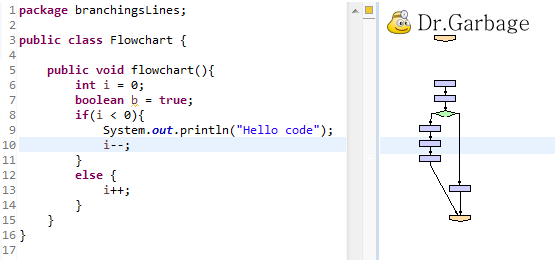
\includegraphics[width=1.00\textwidth]{Figures/Java-flowchart-exp/java-flowchart-example.png}\\[0.1cm]
  \caption[Java sequential block diagram opened in Java Source code Visualizer]{Example of source code visualizer}
  \label{fig:java-flowchart-example}
\end{figure}

A depicted flowchart can be easily extracted into control flow graph (see figure \ref{fig:control-flow-graph}). If there is another similar function, it can be transformed into next control flow graph. These two graphs are being compared using existing TDMC[\ref{sec:topdown}] and BUMC[\ref{sec:bottomup}] algorithms. 

\begin{figure}
  \centering
  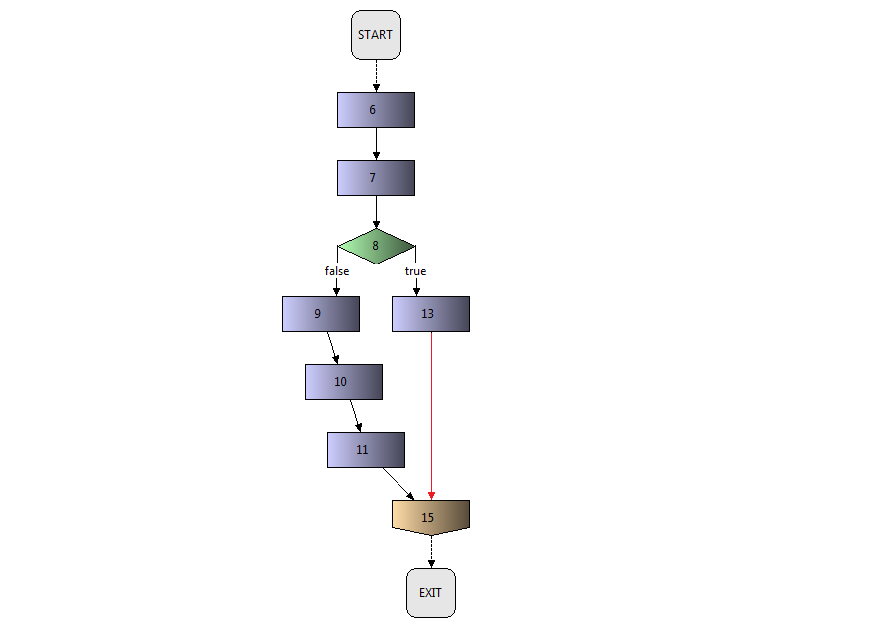
\includegraphics[width=1.00\textwidth]{Figures/Java-flowchart-exp/control-flow-graph.png}\\[0.1cm]
  \caption[Extracted control flow graph from Java source code]{Extracted control flow graph from Java source code}
  \label{fig:control-flow-graph}
\end{figure}

Unfortunately these two algorithms are applicable only for tree structures. For this reason this problem can be reduced, removing minimum number of edges to get a spanning tree. Thus the the edges in the input graphs are reduced by Spanning Tree Algorithm[\ref{sec:graph-transformation}]. The removed edges are red highlighted, hence this for this structure TDMC and BUMC[\ref{cha:algorithms-to-compare}] can be easily applied.

To conduct an experiments a sequence of actions and following statistic are needed. After conducted experiments, taking into account the derived statistic, a conclusion takes place. The steps are carried through sequence of action:
\begin{itemize}
	\item Write two similar functions in Eclipse IDE
	\item Apply for them text-to-text comparison
	\item Declare the statistic, respectively how many lines are different		
	\item Create a source-code graph for both
	\item Apply TD \& BU algorithms to get structural difference	
	\item Declare the statistic, respectively how many nodes are different			
\end{itemize}

In this section all experiments have been executed by hand using plug-in tool "Graph Comparison" in Eclipse from dr. Garbage project. Before starting, a several rules how to evaluate code difference in text and in graph must be established. It is one of the crucial moment, because followed data statistic are used in further tool development.

For the estimation of structural difference there are criteria listed:
\begin{itemize}
	\item Each java operator is considered as simple node
	\item Changing a conditions of block on the contrary issues 100\% difference of business logic, however the structure stays unchangeable.
	\item Availability of extra variables in second piece of code is calculated by division of number of extra variables to amount of all variables.
\end{itemize}

Mostly all calculations are performed by roughly, because there are many criteria how to evaluate the logic and structure difference. But from this perspective these rules are enough to examine graph's similarity.

For the text difference found via Eclipse tool a criteria to evaluate can be added:
\begin{itemize}
	\item Percentage is computed by number of 
	\item If in one line of code only one symbol has been covered as found, then it is division of one to amount of symbols in this line. 
\end{itemize}

\begin{figure}
  \centering
  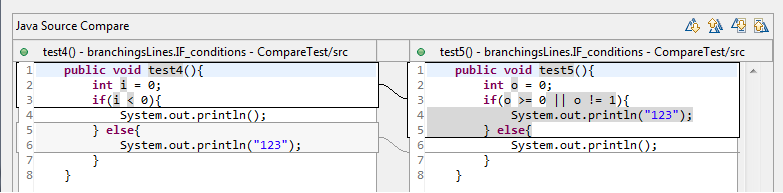
\includegraphics[width=1.00\textwidth]{Figures/Java-flowchart-exp/example-graph.png}\\[0.1cm]
  \caption[Two pieces of code are being compared with Eclipse Text Comparison]{Two pieces of code are being compared with Eclipse Text Comparison}
  \label{fig:example-graph}
\end{figure}

And after generation of two graphs, these both are compared(see the figure \ref{fig:graphs-compared}) using existing TDMC and BUMC[\ref{cha:algorithms-to-compare}] algorithms.
\begin{figure}
  \centering
  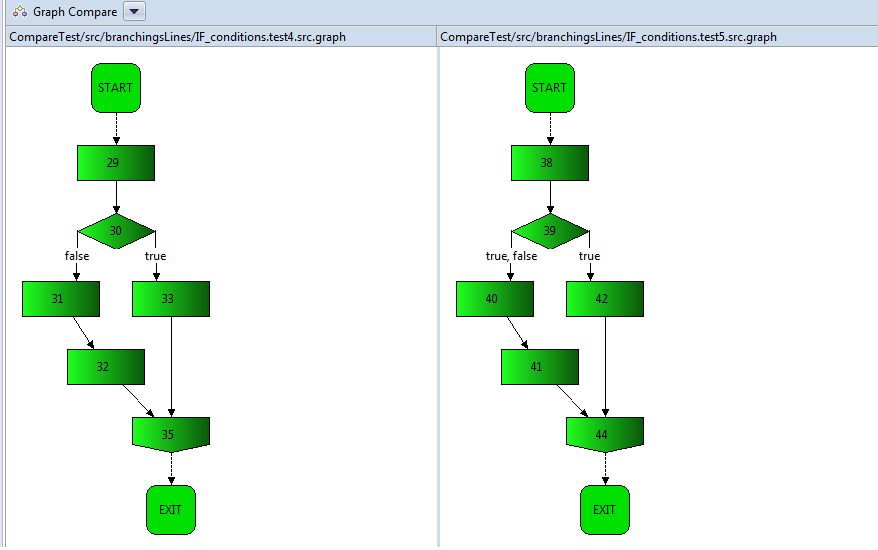
\includegraphics[width=1.00\textwidth]{Figures/Java-flowchart-exp/graphs-compared.png}\\[0.1cm]
  \caption[Compared source code graphs using TDMC algorithm \ref{sec:topdown} ]{Compared source code graphs using TDMC algorithm}
  \label{fig:graphs-compared}
\end{figure}


\begin{table}[h]
\begin{tabular}{|c|c|c|c|c|}
\hline
\multicolumn{3}{|c|}{Compare experiments}                & Text -to-text compared     & Graph compared              \\ \hline
Test id & Name of functions & \begin{tabular}[c]{@{}c@{}}Real  code \\ difference \%\end{tabular} & \begin{tabular}[c]{@{}c@{}}Layout difference\\  \% found\end{tabular} & TD\&BU similarity \% found \\ \hline
1       & t1() and t2() &             50             &             100               &               100             \\ \hline
2       & t1() and t3() &               50           &                   100         &            75                \\ \hline
3       & t1() and t4() &                50          &             100               &              100              \\ \hline
4       & t1() and t2() &                50          &        100                    &                80            \\ \hline
5       & t1() and t5() &                50          &            100                &            100                \\ \hline
6       & t6() and t7() &               33           &                33            &               100             \\ \hline
7       & ti1() and ti2() &              10            &                100            &             0               \\ \hline
8       & ti2() and ti3() &             16             &                100            &              100              \\ \hline
9       & ti3() and ti4() &               25           &         100                   &                 66           \\ \hline
10      & ti4() and ti5() &                 50         &           100                 &                   0         \\ \hline
11      & ti6() and ti7() &                 90         &           100                 &                   42         \\ \hline
\multicolumn{3}{|c|}{Overall results:}                & 93.9 \%  &  69\% \\ \hline

\end{tabular}
\caption{The table demonstrates results of Java Source comparison using text-to-text compare method and application of algorithms to their source code graphs }
\label{table:tests-table}
\end{table}

The table \ref{table:tests-table} shows results of java source code experiments. Existing algorithms [\ref{cha:algorithms-to-compare}] and Eclipse text-to-text comparison have been used to reveal the best approach of code comparison. As it said above, the difference code can be figured out either structurally or simple text comparison. Based on the table \ref{table:tests-table} the apparent conclusion are composed:

\begin{itemize}
	\item If the application logic is totally different (For example \textbf{if conditions}) then Eclipse Text Compare finds the difference, thus condition itself is highlighted. The graphical comparison with TD\& BU are not able to see this distinction. It is obvious since graph theory in this case is able to find 
how similar structure of code fragments. The conducted example \ref{fig:graphs-compared} above can testify this conclusion. In this way graph theory is not applicable to differentiate logic of application.
	
	\item In opposite said above, the graphical compare is quite useful instrument to investigate a code structure. For example, if another third party person has changed local variables, the structure remains same, thus TDMC\& BUMC (especially TDMC) find high level of similarity. Unfortunately this approach is not enough to build a new concept allowing to investigate the difference more precisely.
	
	\item The graph is totally bound to lines of codes. If one brace is shifted, then it's considered one more block in the graph(Dr. Garbage Source Code Visualizer \cite{drgarbage} generates extra node for each code operator). Hence TDMC is not able to find following branch where there an extra node and generated Java source code graph is not optimized for comparison.
	
	\item Text-to-text compare is enough to investigate a text difference because this tool finds every different sub-string in code line. But as stated above, changing variables, sequence of operators or even production same loops with different operators the text-to-text compare find too much unmatched strings. Eventually the result of text compare looks like a disorder with same and unmatched sub-strings.  	
	

\end{itemize}

% JAVA AST TREE CODE EXPERIMENTS
\section{Experiments using Abstract Syntax Tree graphs}

In this section the abstract syntax trees are generated from Java source code using Dr. Garbage plugins \cite{drgarbage}.
The most notable advantage of building AST trees is a direct converting Java source code into AST tree, thereby avoiding graphs with cycles. Thus there is no need to delete back edges(see Spanning tree algorithms).

TODO: short explanation about AST how it looks like and we need them;

In this section all experiments have been executed by hand using plug-in tool "Graph Comparison" in Eclipse from dr. Garbage project \cite{drgarbage}.  Before starting, a several rules how to evaluate code difference in text and in graph must be established. It one of the crucial moment, because followed data statistic are used in further tool development.

TODO: after this compares write a conclusion what is better to compare



% JAVA BYTE CODE EXPERIMENTS
\section{Experiments on JavaByte Code}
\label{sec: java-code-experiments}

In this section an investigation regards java byte-code comparison is expound. Unlike Java source code, the corresponding byte code has practically no application logic. In spite of this the topic must be researched for the clone detection.

\begin{figure}[h]
  \centering
  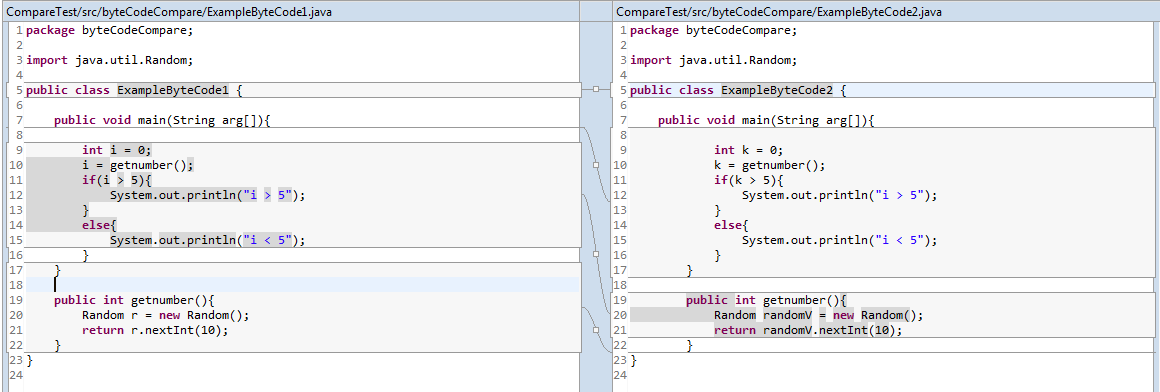
\includegraphics[width=1.00\textwidth scale = 0.9]{Figures/bytecode-compare/example-of-bytecode-original-compared}\\[0.1cm]
  \caption[Functions compared by members]{Java source code compared using text-to-text}
  \label{fig:example-of-bytecode-original-compared}
\end{figure}


\begin{figure}[h]
  \centering
  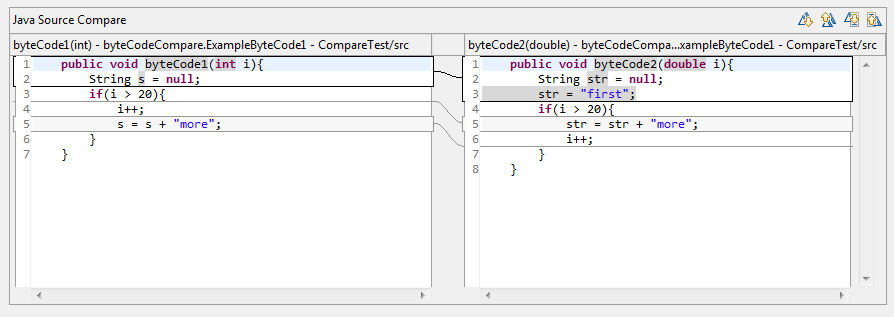
\includegraphics[scale = 0.55]{Figures/bytecode-compare/example-of-bytecode-text-compared}\\[0.1cm]
  \caption[Functions compared by members]{Java byte code compared using text-to-text compare in Eclipse environment}
  \label{fig:example-of-bytecode-text-compared}
\end{figure}

%-----------------------------------------------------
% 5th Chapter: Graph transformation algorithms
%-----------------------------------------------------


\chapter{Graph transformation algorithms}
\label{cha:graph-transformation}

\section{Introduction to the graph transformation}
\label{sec:graph-transformation}

TODO: explain how graph is generated, which libraries are used, plugins

\section{Techniques to normalize AST improving structural comparison}

Researches show that many big development projects have duplicate code, which is generally result of copying and pasting existing pieces of code. Moreover the code can be completely redone, changing name of variables, in some cases replace lines of code. But the most sophisticated part comes when a similar command can be in code substituted. It is known, that from programming perspective, for instance, a loop can be differently organized. There three fundamental ways to reproduce the iteration statements, namely: \emph{pre - condition}, \emph{post - conditions} and so-called \emph{for-loop}. The function can be reworked by so delicate way, that none of any text-to-text compare finds similarity. However the functions execute the same application logic. And this can be found almost everywhere, the most notable example is clone pair between FreeBSD and Linux. 

TODO: write that in for trees this transformation can be applied:\\
Karp-Rabin fngerprinting algorithm is used for calculating the fingerprints of all
length n substrings of a text. First, a text-to-text transformation is performed on the con-
sidered source le for discarding the uninterested characters. Following this the entire text
is subdivided to a set of substrings so that every character of the text appears in at least
one substring. After that the matching substrings are identifed. In that stage, a further
transformation is applied on the raw matches to obtain better results. Instead of applying
a set of text-to-text transformations, he applies several different transformation scenarios
from a combination of basic transformations such as  For ifnding near-miss duplication he
attempted to find a normalized/transformed text by removing all whitespace characters
except line separators and by replacing each maximal sequence of alphanumeric characters
with a single letter 'i'. For example, a line for(k = 1; k <= n; k + +)f" is replaced by
the line i(i = i; i <=; i + +g" and the line hash defineXDEF234" by hash iii".
TODO:
\\

TODO: write from what this idea comes from: section token based technique: normalization
Further research can also be carried out upon cantilever structures or continuous structures.

In the following example \ref{listing1} these functions are similar and have same application logic. If these functions are compared with text compare, then definitely one line with increment of variable \texttt{frameGroupLine} is highlighted. 
\newpage
\begin{lstlisting}[caption={Clone pair between FreeBSD and Linux}, label = listing1]
public void test1(){
		int frameGroupLine = 10;
		for(int Cnt = 1; Cnt < frameGroupLine;  Cnt =+ 2)
		{
			if(Cnt*4 != 2){
				frameGroupLine++;
			}
		}
	}
	
public void test2(){
		int frameGroupLine = 10;
		for(int Counter = 1; Counter < frameGroupLine;  Counter =+ 2)
		{
			if(Counter*4 != 2){ 
				frameGroupLine = frameGroupLine + 1;
			}
		}
	}	
\end{lstlisting}

If this line \texttt{frameGroupLine = frameGroupLine + 1;} will be converted into one format of sub-tree, that indicates the same as \texttt{frameGroupLine++;}. Thus this sub-tree can be found with TDMC or BUMC algorithms. Consequently it brings more covered nodes that signalize more similarity. 

\begin{lstlisting}[caption= {Normalized function \texttt{test3()} concerning variable \texttt {frameGroupLine}}, label = listing1]
	public void test3(){
		int frameGroupLine = 10;
		for(int Counter = 1; Counter < frameGroupLine;  Counter =+ 2)
		{
			if(Counter*4 != 2){ 
				frameTeamLine++;
			}
		}
	}
\end{lstlisting}

In the function \texttt{test2()} one the increment of variable \texttt{frameTeamLine} is differently written. From text to text compare the functions are different at this point. If the text code similarity will be calculated, then these two fragments are not same (probably $90\%$ similarity). Using Abstract Syntax Trees Optimization, this types of structure can be converted in the same sub-tree of whole AST tree. Thereby these two different text structures are represented as same sub-tree. 

\vspace{4mm}

\begin{figure}[h]
  \centering
  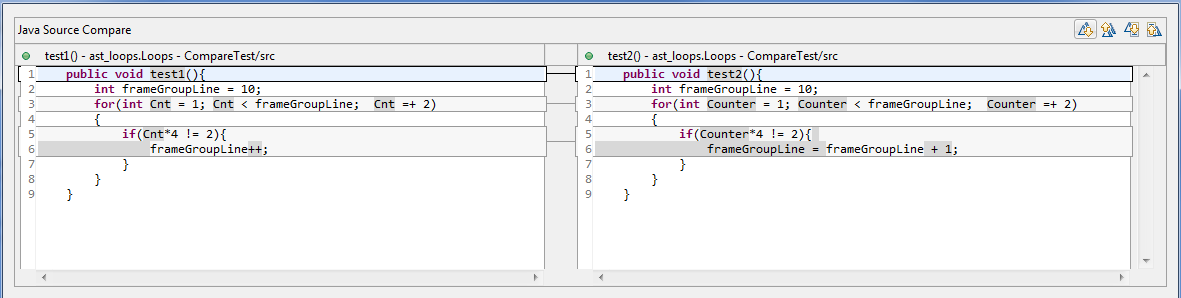
\includegraphics[width=1.00\textwidth]{Figures/AST-optimization/text-to-text-compare}\\[0.1cm]
  \caption[Text to text comparison example]{Example of standard text-to-text comparison of Java code}
  \label{fig:text-to-text-compare}
\end{figure}

On figure \ref{fig:text-to-text-compare} the example demonstrated how these two functions are compared using Eclipse Text comparison window. After creation and comparison these two AST trees, it can be easily seen that sub-trees (the increment) are different.

\begin{figure}[h]
  \centering
  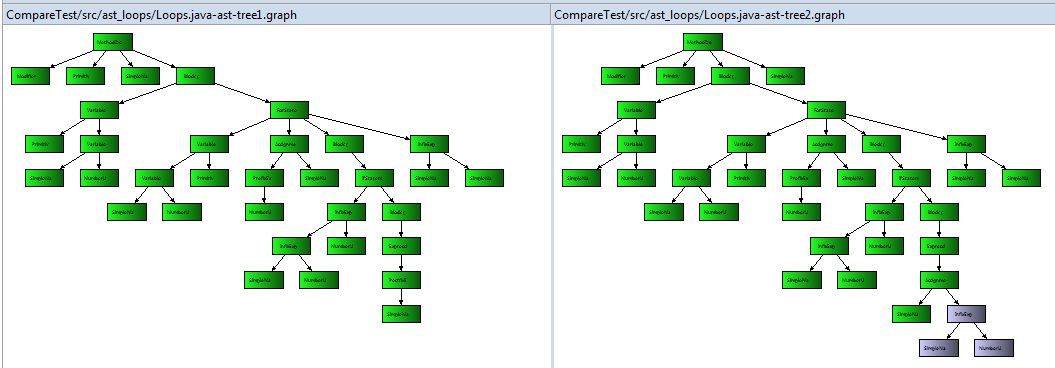
\includegraphics[width=1.00\textwidth]{Figures/AST-optimization/tree-compared1}\\[0.1cm]
  \caption[Graph comparison on similar AST trees]{Graph comparison of function test1() and test2() using TDMC algorithm \ref{sec:topdown}}
  \label{fig:ast-graph-compare-similar-tdmc}
\end{figure}

From the figure \ref{fig:ast-graph-compare-similar-tdmc} TDMC algorithm finds incomplete code similarity since not all nodes have been covered. From statistical point of view using simple math, the percentage of similarity is figured out: 37 nodes in the \texttt{test2()} and 3 of them are not covered. Thus, the calculation indicates  $\left ( 1 - \left (\frac{3}{37} \right ) \right )\cdot 100 = 91\%$ code similarity according to AST trees and applied TDMC algorithm.

This mismatch can be optimized during AST tree production. These two lines of code \texttt{frameGroupLine++;} and \texttt{frameGroupLine = frameGroupLine + 1;}
must be built as a same sub-tree, accordingly same structure and same number of nodes. Using this simple replacement it allows to built a similar AST trees, when logic is same but the source code text is different. Consequently the converted AST trees to some extent are independent from source code and can be compared to explicit the difference.

The example described above is relatively small, but exact showing how this logic can be circumvented. Also in pre-processing of AST tree can be included all possible java operators. This process called code normalization, and can be prepared before the AST tree will have been built. \\

\begin{table}[h]
\centering 
\begin{tabular}{|l|l|l|}
\hline
     Operator                        & input   & output     \\ \hline
\multirow{2}{*}{postfix}     & \texttt{i++}     & \texttt{i = i + 1  }  \\ \cline{2-3} 
                             & \texttt{i--}     & \texttt{i = i - 1  }  \\ \hline
\multirow{2}{*}{prefix}      & \texttt{++i}     & \texttt{i = i + 1 }   \\ \cline{2-3} 
                             & \texttt{--i }    & \texttt{i = i - 1}    \\ \hline
\multirow{7}{*}{assignments} & \texttt{i *= n } & \texttt{i = i * n } \\ \cline{2-3} 
                             & \texttt{i /= n  }& \texttt{i = i / n } \\ \cline{2-3} 
                             & \texttt{i \%= n }& \texttt{i = i \% n }\\ \cline{2-3} 
                             & \texttt{i -= n } & \texttt{i = i - n } \\ \cline{2-3} 
                             & \texttt{i += n  }& \texttt{i = i + n } \\ \cline{2-3} 
                             & \texttt{i =+ n } & \texttt{i = i + n}  \\ \cline{2-3} 
                             & \texttt{i =- n } & \texttt{i = i - n } \\ \hline
\end{tabular}
\caption{The table demonstrates proper string transformation for AST tree optimization. In event of occurrence  of input operator, the original can be substituted before AST tree have been built.}
\label{table:operators}
\end{table}

The table \ref{table:operators} presents possible java string transformation depending on the input command. Thus the fragment of code will be better prepared for AST tree reformation. The trees of both both comparing functions will more similar that TDMC algorithm finds more similarity. Using statistical data to consider how function similar to each other the formula can be derived. Let $NC$ is subset all of unmatched nodes then\\
$ N \subseteq T_{1}: n \in NC $ and $ M \subseteq T_{2}: m \in NC $ \\
The trees are combined as set of vertexes and edges, thereby $T_{1} = (V_{1}, E_{1})$ and $T_{2} = (V_{2}, E_{2})$ respectfully, the the probability that two functions have same structure takes place: \\
\begin{gather*}
similarity(\%) =  \left ( 1 - \left (\frac{max(|N|, |M|)}{max(|V_{1}|, |V_{2}|)} \right ) \right )\cdot 100 
\end{gather*} \\
where $|V_{1}|$ and $|V_{2}|$ are cardinalities of their subsets. In other words the formula can be described as ratio of maximum number of unmatched nodes between $T_{1}$ and $T_{2}$ to maximum number of nodes in both trees $T_{1}$ and $T_{2}$. 

TODO: derive how it is possible to built same types of loops, (IDEA read about tockens techniques)

\section{Convert graph to tree}
\label{sec: generate-to-tree}
TODO: decribe here how to remove edges in order to get spanning tree, DO WE NEED IT HERE??


\section{Text comparison improvement with AST trees}
\label{sec:text-improvement}
%HOW TO IMPROVE TEXT TO TEXT COMPARE WITH AST TREES
IDEA: how search for precise difference using AST trees and reflect this to text
\begin{figure}[h]
  \centering
  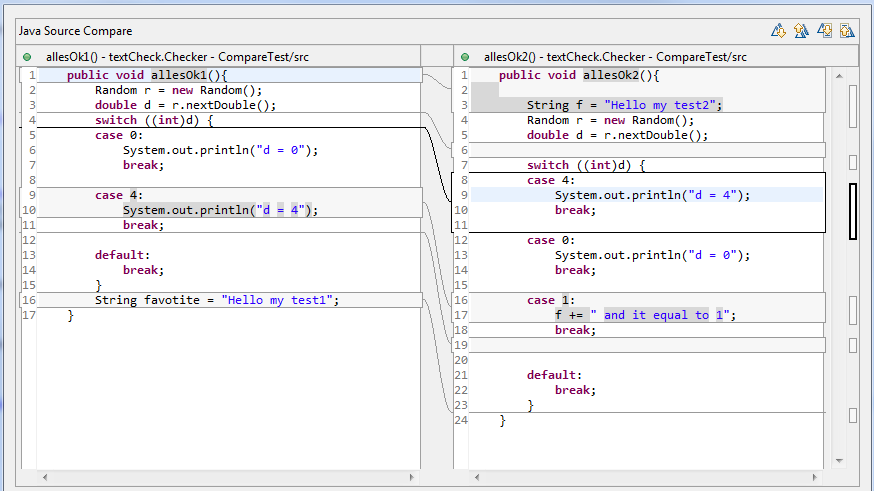
\includegraphics[scale = 0.5]{Figures/text-to-text/text-compare-shifted.png}\\[0.1cm]
  \caption[Text to text comparison example not optimized]{Example of standard text-to-text comparison of Java code}
  \label{fig:text-to-text-compare-shifted}
\end{figure}

This example \ref{fig:text-to-text-compare-shifted} demonstrates how text compare is not available to notice the string difference in case some operators have been simply replaced. Namely the operators: \texttt{case 0:} and \texttt{case 4:} from figure \ref{fig:text-to-text-compare-shifted} have been replaced but text compare find this difference. Moreover when this code mostly changed, namely the names of variable, line position in code, thereby not impacting on the application logic of function then it is much more difficult to clarify the code difference. Thus comparing two function using text to text compare, it can be that the result is totally mixed, however this functions almost identical.
\\
Why text-to-text cannot find these obvious differences? This algorithm for string search is described in chapter \ref{sec: text_tech}. Using suffix tree algorithm  According to research of Roy, Chanchal Kumar \cite{software_clone_detection} there are some disadvantages that can interpret the issue described above on picture \ref{fig:text-to-text-compare-shifted} where some sub-strings are not found described in following citation:
\begin{quote} 
This tools does not support exploration and navigation through the duplicated code. Detection accuracy is low e.g., cannot detect code clones written in different coding styles. For example "\{" position of if-statement or while-statement. Cannot detect code clones using different variable names, e.g., we want to identify the same logic code as code clones even if variable names are different\cite{software_clone_detection}. 
\end{quote}

Hypothesized that tree suffix algorithm is more negatively related to proper code compare in case if clone detection is being searched. 
This can be improved with help of tree algorithms techniques;
%IDEA!!
\begin{figure}[h]
  \centering
  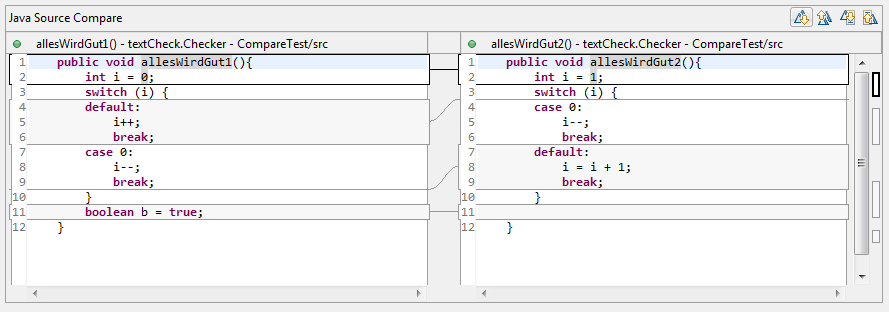
\includegraphics[width=1.00\textwidth]{Figures/text-to-text/text-compared-for-improve}\\[0.1cm]
  \caption[Text to text comparison example when lines of code are replaced]{Example of text-to-text demonstrating the code difference using sub-suffix algorithm }
  \label{fig:text-compared-for-improve}
\end{figure}
As prerequisites let us take the following example depicted on the picture\ref{fig:text-compared-for-improve}. Considering the example very carefully, line by line, it is easy to get an idea how these two peaces of code organized. In line 2 the obvious mismatch variable \textbf{\texttt{o:1}} to \texttt{0} and \texttt{false} to \texttt{true} are gray highlighted.
Up next comes the \texttt{if} operator, where there are two and three blocks. They make almost the same logic however the ae The last difference on line 11: function \texttt{test2()} contains extra command \texttt{b = true;}.
At the end of function \texttt{test2()} there is additional operator. Notice that, the example is relatively small and has not some much different commands and operators. It can be that two functions are so complex modificated, thereby text compare yields a mix of various lines. To improve this, a code can be transformed into Abstract Syntax Tree(next AST tree) and both tree are traversed synchronously checking matched nodes. The biggest advantage of method that AST trees are built independently of sequence of commands. The difference in this trees is unordered range of nodes. It means that these AST trees are taken into consideration as unordered trees.

\begin{figure}[h]
  \centering
  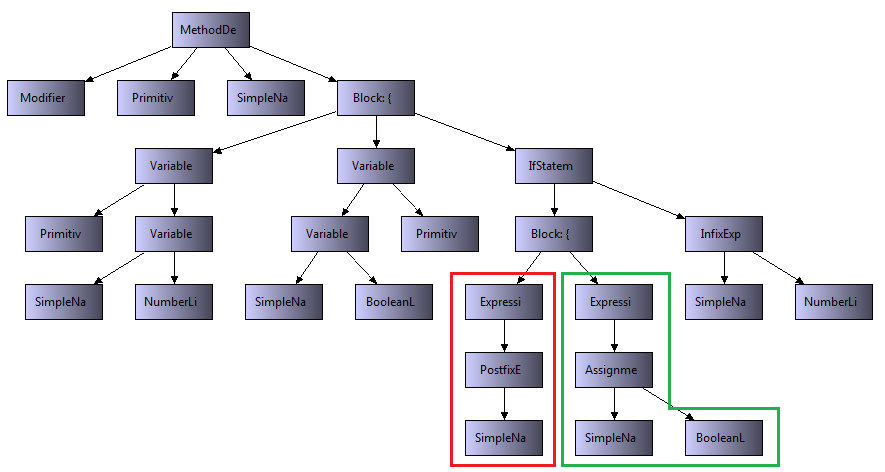
\includegraphics[width=1.00\textwidth]{Figures/text-to-text/graph-compared1.png}\\[0.1cm]
  \caption[Abstract Syntax Graph  of function \texttt{test1()}]{Abstract Syntax Graph  of function \texttt{test1()}.}
  \label{fig:graph-compared1}
\end{figure}
The picture \ref{fig:graph-compared1} shows how AST tree from function \texttt{test1()} is being built from the source code. As said above the presented AST tree \ref{fig:graph-compared1} is unordered, thus the replaced lines of code and the nested operators and independent from each other. The trees traversal enables to identify the concrete difference in source code, independent how the code is organized. The evident mismatch must be referred to the source code. The idea is to keep the current command or operator in the tree node, i.e. to keep to current text position of command in the corresponding node. Obviously the proper node forming is kept during the AST tree convert process. After complete parallel tree traversal similar to Breadth-first search, the nodes of $i$ level are compared for matched content, in this case operators and command. If in the level  $i$ a match if not found, the mismatched nodes are marked as mismatch. Each node contains information about text location of command or operator. During the second tree traversal on trees when mismatched node is visited, the corresponding text is highlighted in text compare. Therefore it helps to improve standard text-to-text compare.
\\
\begin{figure}[h]
  \centering
  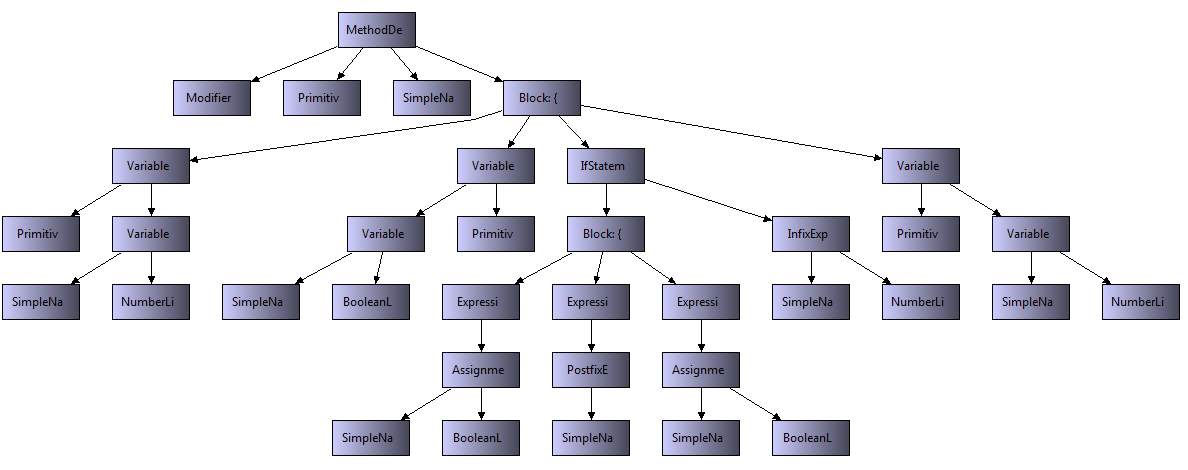
\includegraphics[width=1.00\textwidth]{Figures/text-to-text/graph-compared2.png}\\[0.1cm]
  \caption[Abstract Syntax Graph  of function \texttt{test2()}]{Abstract Syntax Graph  of function \texttt{test2()}.}
  \label{fig:graph-compared2}
\end{figure}

Example \ref{fig:text-compared-for-improve} and derived AST trees \ref{fig:graph-compared1} and  \ref{fig:graph-compared2} indicate similarity and difference: the red and green framed branches are same(\texttt{i++} and \texttt{b = false }respectfully), therefore the nodes in this branch are marked \emph{matched}. The yellow frame marks out \texttt{b = true;} line, that is redundant in \texttt{test1()}. Since the trees are unordered and running over all nodes in $test1()$ and $test2()$ tree structure at same node depth level $i$ using Cartesian Product among nodes search for different or missed nodes and mark them as mismatch.
\\
TODO: write math formula taking i nodes and Cartesian set
\\

The blue frame in picture \ref{fig:graph-compared2} denotes a new command line, namely \texttt{double d = 1.1;}. In Cartesian product this parent node must be not matched, hence the whole branch is marked as mismatch. \\
TODO: example which strings must be highlighted in text as a reflex to mismatched nodes.
\\
%IDEA 2
Possible IDEA 2
After second tree traversal to see the mismatch, a non-trivial statistic takes a place:
Show in what parts of code the changes has been detected, For example: 
\begin{itemize}
	\item Conditions have been changed (percentage )
	\item Code added /removed (percentage )
\end{itemize}

%IDEA 2
%IDEA 3: to compare inside the nodes suffix tree algorithm takes place
%-----------------------------------------------------
% 6th Chapter: Graph transformation algorithms
%-----------------------------------------------------
\chapter{Existing Comparison methods}
\section{Plagiarism detection methods}
\label{sec: plagiarism_methods}

Task of plagiarism detection is an identification of text's similarity. Thus a research of existing methods is useful for this work regards code's comparison.
\begin{quote} Plagiarism detection is the process of locating instances of plagiarism within a work or document. The widespread use of computers and the advent of the Internet has made it easier to plagiarize the work of others. Most cases of plagiarism are found in academia, where documents are typically essays or reports. However, plagiarism can be found in virtually any field, including scientific papers, art designs, and source code \cite{wiki_plagiarism}. \end{quote}

Mostly the task of plagiarism detection is considered for many fields, like text documents, software and source code. In this chapter source code plagiarism is being reviewed.

According to the article of Chanchal Kumar Roy and James R. Cordy \cite{software_clone_detection}, source-code similarity detection 
algorithms can be classified as following:
\begin{itemize}
	\item Text-based Techniques
	\item Token-based Techniques
	\item Tree-based Techniques
	\item PDG-based Techniques
	\item Metrics-based Techniques
\end{itemize}
According to this research the above methods are described in this chapter. The following conclusion takes a place to overview pros and cons of these methods and 


\section{Text-based Techniques}
\label{sec: text_tech}

Text based techniques are widely used to compared pieces of text. For this purpose they can be valuable to compare java source code. This section shortly explains how it functions and derived advantages and disadvantages from chapter experiments \ref{cha:experimental}. Used technique in text-to-text comparison applies so-called tree suffix algorithm, designed to compare strings. General idea of this suffix tree comparison algorithm: the code is splitted into strings, from these strings a suffix tree is being built, then using sub-suffix algorithm performs a search for substring from one code fragment to another. Building such kind of tree allows to find a sub-string in given string within $O(m)$ complexity, where m is the length of the sub-string (but with initial $O(n)$ time required to build the suffix tree for the string). 
\\
TODO: suffix tree example
Thus the algorithm is being applied for normalized text after steps above. The text comparison splits each $i$ line of code and compare the string with $i$ line of code of other fragment. From the first string the suffix tree is built. The second line of code as a search-string is interpreted. The suffix tree is traversed looking for search string occurrence. From performed experiments from chapter of experiments \ref{cha:experimental} the next conclusion can be derived. \\
Advantages of text-to-text comparison:
\begin{itemize}
	\item The difference direct in text represented.
	\item Every small mismatch is noticed and highlighted.
	\item High performance due to optimal formed suffix tree, that the match of search string is for $O(m)$ complexity executed, where $m$ is length of searched sub-string.
\end{itemize}
Disadvantages of text-to-text comparison:
\begin{itemize}
	\item If lines of the same command are different, comparison says it is mismatch.
	\item Changing the order of command or variable's names bring almost full mismatch.
	\item If sequence of commands and names of variable have been changed or modified then text highlight result is too jumbled.
\end{itemize}

In order to avoid line's mess, the graph theory can be very helpful to make application logic more independent from text, therefore to improve quality of text difference representation. The paragraph \ref{sec:text-improvement} interprets an idea how AST tree assists to specify precisely match/mismatch of command .

\section{Token-based Techniques}
\label{sec: tocken_tech}

Using this technique the input code is firstly prepared with lexical analyzer. The entire code is lexed, parsed and transformed into sequence of tokens. This principle is advanced text-to-text comparison concept with steps before text comparison starts the preparation of code includes following steps:
\begin{enumerate}
  \item Comments Removal: Ignores all kinds of comments in the source code depending on the language of interest.
  \item Whitespace Removal: Removes tabs, and new line(s) and other blanks spaces.
  \item Normalization: Some basic normalization can be applied on the source code.
\end{enumerate}

One of the leading token-based techniques is CCFinder from Kamiya\cite{tocken_kamiya}. Firstly, each line of source files is divided into tokens by a lexer and the tokens of all source files are then concatenated into a single token sequence. The token sequence is then transformed, tokens are added, removed or changed based on the transformation rules of the language of interest aiming at regularization of identifiers and identification of structures. 
After that each identifier related to types, variables, and constants is replaced with a special token\cite{tocken_kamiya}. This identifier replacement makes code fragments with different variable names clone pairs \cite{tocken_kamiya}. A suffix-tree based sub-string matching algorithm is then used 
to the similar sub-sequences on the transformed token sequence where the similar sub-sequence pairs are returned as clone pairs/clone classes\cite{tocken_kamiya}. When the clone pair class is obtained according to the token-sequence, the original code must be mapped regards to clone pair/clone class information.
\begin{enumerate}
  \item \textbf{Lexical analysis} - each line of code is divided into tokens depending on programming language. The tokens are parsed via lexical analyzer which performs formatting of tokens, the rules described above reconstructing the source code is.
\item \textbf{Transformation}  - the process includes two sub-processes. During the sub-processes the meta information regards mapping to original source code is kept. Thus the original code is restructured without loss of link-identifiers.
  \begin{enumerate}[label*=\arabic*.]
    \item \textbf{Transformation according to determined rules} - the token sequence is reorganized pursuant to some rules. One of them is conversion of compound block. For example the code: \texttt{if(i == 1) i = i + 1;} is being transformed into: \texttt{\textbf{if(i == 1) \{i = i + 1;\}}} covered within brackets. All other rules can be programming language dependent.
    \item \textbf{Parameter replacement} - each identifier related to types, variables and constant is replaced with special token\cite{tocken_kamiya}.
  \end{enumerate} 
  \item\textbf{Match detection} - the token sequences are searched for equivalent pairs and marked as clones with suffix-tree algorithm [\ref{sec: text_tech}]. Each clone is divided by indices in four parts: LeftBegin, LeftEnd, RightBegin, RightEnd. These metrics are indices of leading clone for mapping for according positions in the following clone.
  \item\textbf{Formatting} - the clones in original code are highlighted according results from previous step.
\end{enumerate}
These results followed by \cite{tocken_kamiya} provide confirmatory evidence that native text comparison [\ref{sec: text_tech}] can be significantly improved. Simple based normalization of code structure, namely transformation in tokens,  brings better results as compare to native text comparison [\ref{sec: text_tech}]. 


\section{Tree-based Techniques}
\label{sec: tree_tech}
The research from Chanchal Roy \cite{software_clone_detection} offers an alternative to figure out differences using trees. The complex trees are formed from source code and parsed to find mismatched nodes. The most remarkable distinction between text-to-text compare and trees is logic of tree building. In other words, the text compare assumes also a suffix-tree creation, however this technique is based on input strings, i.e the structure of the tree depends on letters and sub-string\ref{sec: text_tech}. The alternative approach is tree creation directly from source code, based on programming language. It encompasses building a branch of trees not by one string line, but by a combination of programming command structures. Such logic of tree creation called Abstract Syntax Tree (in short, AST). The abstract syntax tree analysis is more accurate than a line by line analysis or programming language token based approach \ref{sec: tocken_tech} due to the fact that it builds the abstract syntax tree.\\
The proposed clone detection solution from \cite{flavius} can be organized into few steps:
\begin{enumerate}
	\item Parsing via source code and create non-optimized AST tree.
	\item Each sub-tree of AST tree is hashed and grouped by in different buckets based on their hash value. 
	\item Apply the clone detection algorithm that three sub-algorithms:
		\begin{enumerate}[label*=\arabic*.]
		\item Basic Algorithm finds sub-tree clones compares every sub-tree with another sub-tree for equality. The algorithm uses parsing both AST trees finding out clones with exact equality and excludes the possibility to find near-miss clones. The complexity of algorithm offered from Baxter \cite{baxter} is 
$ O(N^3)$. This can be reduced using hash-value in node parents of sub-tree. Thus each parent node keeps a hashed value about sub-tree itself. For example, a parent node contains following tree structure: \texttt{for(int i = 1; i <= 10; i++ )\{ b = b + 1; \}} that represents a complex sub-tree. The hash-value of structure is \texttt{f4caf1dd3e33c53d971f0e18f72249e0}. During tree traverse the hash values of corresponding nodes are compared. If these hash values are same there is no need to check the whole sub-tree. Otherwise sub search is being further proceed. This technique is used to optimize search of equal sub-structures between AST trees. In most cases it contributes up to $30\%$ performance, since searched projects keep clones.
		\item Sequence Detection - is a part of clone detection the algorithm that handles the detection of code clones within sequences of statements or declarations \cite{flavius}. When parsing a source code fragment, all sequences are stored in a sequence list for future usage. The first step named subsequence algorithm, takes care of detecting code clones inside each sequence, and verifies if two sub-sequences of the same sequence are clones.	
		\item Generalization algorithm - the algorithm takes care about detection near-miss clones. It verifies whether the parent nodes of detected clones belong to near-miss clones.
		 \end{enumerate} 
\end{enumerate}

\begin{figure}[hb]
  \centering
  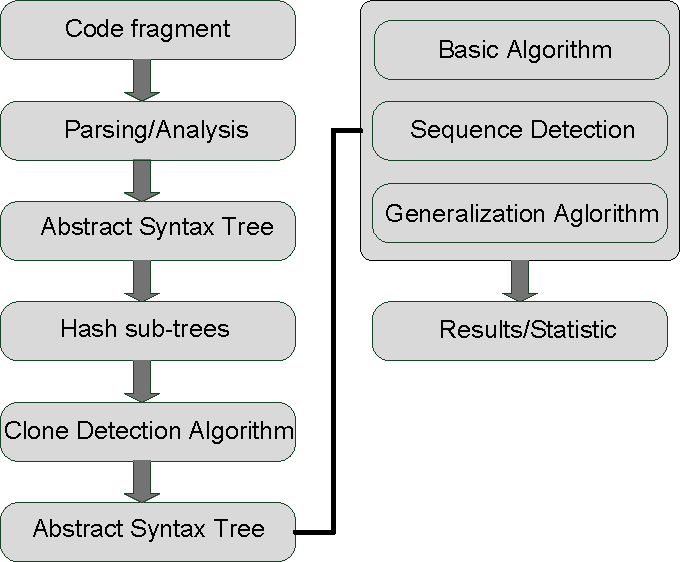
\includegraphics[scale=0.75]{Figures/exist-alg/ast-scheme2.pdf}\\[0.1cm]
  \caption[General steps of code comparison with AST tree]{The flowchart demonstrates general steps of code comparison with AST trees. Once the Abstract Syntax tree has been created, a sequence of algorithms is applied.}
\end{figure}

In summary, tree-based approach is the most flexible tool to compare source code because only this fragment of code has a syntax and structure. Consequently a flexible tree can be built based on syntax itself. \\
Advantages of Abstract syntax tree comparison:
\begin{itemize}
	\item Possibility to investigate for clones in sub-expressions on highest abstract level
	\item Semantic analysis during tree assembling 
	\item Independence form comments, spacing, or other non-semantic changes
\end{itemize}
Disadvantages of Abstract syntax tree comparison:
\begin{itemize}
	\item Execution time, comparing sequences of trees the computational process is $O(N^4)$. But due to hashing of buckets it can be significantly reduced.
	\item Complexity of algorithms to parse trees and figure out clones.
	\item So far this algorithm have been used only to identify clones and add/remove sequences of clone to optimize projects. For small examples of code there are yet an algorithm to represent clones textually. This concept is described in section \textbf{Text comparison improvement with AST trees} \ref{sec:text-improvement}.
\end{itemize}
As described above it allows to differ even small clones between two pieces of code. This technique is not suitable for pure text since text has no logic and structure. AST tree based technique is not fit with Java Byte code since Java byte-code has not so much complex structure to form an AST tree.


\section{PDG-based Techniques}
\label{sec: pdg_tech}
PDG based techniques for clone detection is most suitable to detect for non-contiguous code clones while other clone detection technique as AST in section \ref{sec: tree_tech}, text and token methods are not. The most remarkable difference of other approaches is logical content of graph, therefore the dependencies among variables and methods. This method sets an effective testing to discover and locate the redundant functional modules and the unreachable paths based on dependency relationship.
\\
A program dependency graph (in short, PDG) is a directed graph $ G = (V, E)$ contains the control flow and data flow and represents the dependencies between program elements (statements). Respectively a PDG nodes $V_{i}$ is a program element and a PDG edge $E_{i}$ indicates a dependency between two nodes. PDG is considered as a combination of two different layer sub-graphs: a data dependence sub-graph (in short, DDS) and a control dependence sub-graph (in short, CDS).
After PDG graph creation, a matching algorithm is applied to find a similar sub-graphs which are returned as clones.


\begin{lstlisting}[numbers=left, numbersep=-5pt]
    private static String sample(){
 		   String text = null;	
		   int i = 0;
		   while(i < 10){
				i++;
				text.compareTo("my text");
				text.trim();
		}
		return  text;
	} 
\end{lstlisting}

\begin{figure}[hb]
  \centering
  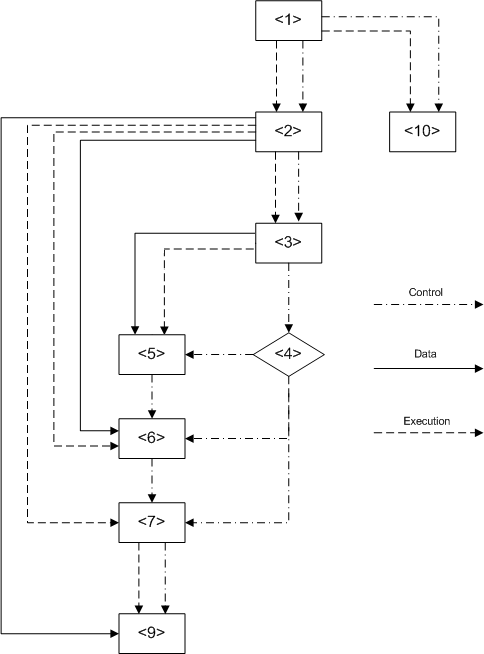
\includegraphics[scale=0.55]{Figures/exist-alg/pdg-example.png}\\[0.1cm]
  \caption[PDG 2]{Program Dependency Graph derived from Java source code}
  \label{fig:pdg-ex}
\end{figure}

Labels attached to the nodes mean the lines where their elements located in the source code. The node labeled <1> is the enter node of the PDG graph. This example example demonstrates data dependencies between nodes using variables. Node $<2>$ has initialization of text variable \texttt{text}, this variable is used in lines 6 and 7, therefore there are edges from node $<2>$ to nodes $<6>$ and $<7>$ respectfully. The dashed line from $<2>$ to $<6>$ and $<7>$ indicates that some methods on this variable used. Moreover the node $<6>$ has data edge because of input parameter of method \texttt{compareTo()}. The loop $<4>$ keeps under execution all actions inside.\\
The algorithm for clone detection offered from \cite{pdg} is based on Komondoor's Method\cite{Komondoor}:
\begin{enumerate}
  \item All nodes are hashed according to their content, similar as in AST tree compare \ref{sec: tree_tech}. Nodes with the same hash value are considered as equivalent class. The hashing process is independent from name of variables, thus only syntactically identical program elements have the same hash value. 
  \item The second step the pair of root nodes of all equivalence classes is identified. In other words roots $(r_{1}, r_{2})$ of similar sub-graphs are explored. If the predecessors $(p_{1}, p_{2})$ have the same hash value, the \textbf{slicing operation} is executed and the predecessors are added into list of pair of slices. 
  There are some cases when these pairs are not added in the list:
  \begin{enumerate}
	  \item Predecessors $(p_{1}, p_{2})$ have different hash values
	  \item Predecessors $(p_{1}, p_{2})$ have the same hash value but $p_{1}(p_{2})$ already in the slice list $r_{1}(r_{2})$. This technique provides an avoiding of endless loop.
	  \item Predecessors $(p_{1}, p_{2})$ have the same hash value but $p_{1}(p_{2})$ already in the slice list $p_{2}(p_{1})$. This technique ensures to prevent two slices from sharing the same node.
	\end{enumerate}
	\item If a clone pair of statements $(s_{1}, s_{2})$ is subsumed to another clone pair $(s_{1}', s_{2}')$ such that the following intersection takes place $s_{1} \subseteq s_{1}' \cap s_{2} \subseteq s_{2}'$. This intersection  is removed from the set of detected clone pairs. This removal must not affect on application logic since these clone pairs are not useful.
	\item The clone set is created from clone pairs as union of clone pairs. For example $(s_{2}, s_{4})$ and $(s_{2}, s_{5})$ generate a set $(s_{2}, s_{4}, s_{5})$.
\end{enumerate}

A program slicing is the union or association of the set of programs statements, that affects the values at some point of interest, referred to as a slicing criterion. Initially it is used for debugging purposes to trace the whole process of concrete data structure. This procedure is used 
in the algorithms described above in step 2. The example reveals slicing operation under function \texttt{mySlice()}:
\begin{lstlisting}
public void mySlice(){
		boolean detected = false;
		int amount = 0;
		String listOfClones = null;
		while(amount < 10){
			amount ++;
			listOfClones += "clone number: " + amount; 
		}
		System.out.println(listOfClones);
		System.out.println(amount);
	}
\end{lstlisting}
The criterion of slicing is variable \texttt{listOfClones} and therefore the new sliced instance is code:
\begin{lstlisting}
public void mySlice(){
		int amount = 0;
		String listOfClones = null;
		while(amount < 10){
			amount ++;
			listOfClones += "clone number: " + amount; 
		}
		System.out.println(listOfClones);
	}
\end{lstlisting}

The algorithm was offered from Komondoor \cite{Komondoor} in his research "Semantics-preserving procedure extraction". The noticeable feature of this whole technique is that the clones in code are searched in the one code fragment itself. This technique of clone detection based on program dependency graphs offered by Yoshiki Higo \cite{pdg} is mainly directed to find clones in the input code of course depending of programming language. Thus there is no second input code chunk can be compared. The idea is code redundancy and optimization of execution in relative large projects when the pasted code is incorrectly changed or forgotten to be changed.
\\
The appreciable privilege of such kind of graphs is obvious. The logical relationship among variables and methods are established in the graph that makes possible to comprehend the information flow control and usability of statements. Unlike the previous ways to find clone like text-to-text \ref{sec: text_tech} or AST trees \ref{sec: tree_tech} are not able to keep statements of elements of statements that are not consecutively located on the source code. However it can be improved with AST tree comparison when same statements are split with regards to their locations in section Text Comparison improvement with AST trees \ref{sec:text-improvement}.
\\
There are some weaknesses of existing PDG based detection methods. Compared to other detection techniques, the first weakness is that PDG-based detection has lower performance for the detection of contiguous code clones \cite{pdg}. This is because consecutive program elements in the source code do not have necessarily data dependency or control dependency. On the other hand, line- or token-based detection methods do not consider such dependencies but rather compare program elements textually, so that these methods are productive at detecting contiguous code clones. 
Secondly the PDG-based detection has a high computational complexity. The number of nodes used as slice point is significantly large and every slice performed operation is a non-trivial task.



%-----------------------------------------------------
% 5th Chapter: Conclusion
%-----------------------------------------------------

\chapter{Conclusion}
\label{cha:Conclusion}

based on experimental results and own opinion, write here what results were derived 
From time to time write here combined conclusions or improvements
Each detection
technique has its own relative advantages and disadvantages, and no technique is superior to any of the other
techniques in all aspects


%-----------------------------------------------------
% Literature
%-----------------------------------------------------

\newpage
%\bibliographystyle{plain}
\begin{thebibliography}{100} % 100 is a random guess of the total number of references 
\addcontentsline{toc}{chapter}{Bibliography}
%Example:
%\bibitem{ch11} George H.L. Fletcher and Catharine M. Wyss, "Data Mapping as Search", Computer Science Department, School of Informatics, Indiana University, Bloomington, USA. 

 \bibitem{drgarbage}The Dr. Garbage Tools Project\textregistered \enspace 2014, Sergej Alekseev, Peter Palaga and Sebastian Reschke, URL:
\url{http://www.drgarbage.com}

 \bibitem{graph_compare} Sergej Alekseev. \emph{ Graph theoretical algorithms for control flow graph comparison}, 2013.
 
\bibitem{valiente} Gabriel Valiente,\emph{Algorithms on Trees and Graphs}, Berlin: Springer-Verlag, 2002.

\bibitem{wiki_flowchart} Free content Internet encyclopedia - Wikipedia: Flowcharts, URL: \url{https://en.wikipedia.org/wiki/Flowchart}

\bibitem{wiki_plagiarism} Free content Internet encyclopedia - Wikipedia: Plagiarism detection, URL: \url{http://en.wikipedia.org/wiki/Plagiarism_detection}
 
\bibitem{software_clone_detection} Roy, Chanchal Kumar; Cordy, James R. (September 26, 2007). \emph{"A Survey on Software Clone Detection Research".} School of Computing, Queen's University, Canada.

\bibitem{graph_isomorphism_is} Koebler Johannes; Schoening, Uwe. (July 29, 1991). \emph{"GRAPH ISOMORPHISM IS LOW FOR PP".} Theoretische Informatik, Universitaet Ulm

\bibitem{baker} Brenda S. Baker \emph{"A Program for Identifying Duplicated Code".} AT\&T Bell Laboratories, Murray Hill, New Jersey

\bibitem{change_distilling} Beat Fluri, Student Member, IEEE, Michael Wuersch, Student Member, IEEE, Martin Pinzger, Member, IEEE, and Harald C. Gall, Member, IEEE \emph{"Change Distilling: Tree Differencing for Fine-Grained Source Code Change Extraction".} Department of Informatics, University of Zurich, Zurich 

\bibitem{tocken_kamiya} Toshihiro Kamiya, Member, IEEE, Shinji Kusumoto, Member, IEEE, and Katsuro Inoue, Member, IEEE \emph{"CCFinder: A Multilinguistic Token-Based Code Clone Detection System for Large Scale Source Code".} July 2002

\bibitem{flavius} Flavius-Mihai Lazar \emph{"Clone detection algorithm based on the Abstract Syntax Tree approach".} Politehnical University of Timisoara, Timisoara, Romania, 9th IEEE International Symposium on Applied Computational Intelligence and Informatics May 15-17, 2014 Timişoara, Romania

\bibitem{baxter} Ira D. Baxter, Andrew Yahin, Leonardo Moura, Marcelo Sant Anna, Lorraine Bier \emph{"Clone Detection Using Abstract Syntax Trees".} Semantic Designs 12636 Research Blvd. Suite C214, Austin Texas

\bibitem{pdg} Yoshiki Higo, Shinji Kusumoto \emph{"Code Clone Detection on Specialized PDGs with Heuristics".}2011 15th European Conference on Software Maintenance and Reengineering - Graduate School of Information Science and Technology, Osaka University, Suita, Osaka, Japan

\bibitem{Komondoor} R. Komondoor and S. Horwitz \emph{"Effective, Automatic Procedure Extraction".}in Proc. of the 27th ACM SIGPLANSIGACT
on Principles of Programming Languages, Jan. 2000, pp. 155–169.

\bibitem{eclipse_site} Eclipse documentation, URL: \url{http://help.eclipse.org/luna/index.jsp}

\bibitem{sample1} Sample Author, NAME,
(Berlin: Springer-Verlag, 2002).

\end{thebibliography} 

\end{document}
